\documentclass[12pt,a4paper,final,oneside]{article}			%definire grandezza testo, foglio e tipo di testo.

%				** TIPI DI DOCUMENTI **
%			- article
%			- book
%			- report
%			
%
\usepackage[utf8]{inputenc}			%definisce la codifica dei caratteri
\usepackage[italian]{babel}				%definisce il pacchetto della lingua
\usepackage{amsmath}						%contiene molti utili strumenti per la scrittura matematica
\usepackage{amsfonts}
\usepackage{amssymb}
\usepackage{makeidx}
\usepackage{graphicx}
\usepackage{lmodern}
\usepackage{units}  					%unita di misura
\usepackage{pgfplots}				%grafici
\usepackage{subcaption}  		%per le figure
\usepackage{gensymb} 			%per i gradi
\usepackage{pst-solides3d}  %per figure in 3D
\usepackage[hidelinks]{hyperref}				%permette di linkare
\usepackage{circuitikz}			%per circuiti
\usepackage{pgfplots}				%per fare plot pgf
\usepackage{subcaption}		%DON'T KNOW. INVESTIGATE
\usepackage{siunitx} 				%unita SI
\usepackage{wrapfig}				%per mettere più immagini insieme
\usepackage{bbold}					%per avere numeri in \mathbb{}
\usepackage{mathrsfs}			%per usare cose tipo \mathscr{}
\usepackage{physics}				%contiene molta notazione utile; lo uso in particolare per \bra e \ket
\usepackage{pgfplotstable}	%DON'T KNOW. INVESTIGATE
\usepackage{titlesec}				%per formattare titoli, paragrafi etc.
\usepackage{csquotes}
\usepackage[final]{pdfpages}    % Per poter includere altri pdf
\usepackage{scrextend}      % Per poter usare footref
\usepackage{multicol}       % per usare più colonne
\usepackage[margin=2.2cm]{geometry}        % per definire la geometria del foglio
\usepackage{movie15}
\PassOptionsToPackage{hyphens}{url}
\usepackage{hyperref}    % Per forzare gli url ad andare a capo
\usepackage{afterpage}

\newcommand\blankpage{%
    \null
    \thispagestyle{empty}%
    \addtocounter{page}{-1}%
    \newpage}



% Serve per le footnotes
\makeatletter
\newcommand\footnoteref[1]{\protected@xdef\@thefnmark{\ref{#1}}\@footnotemark}
\makeatother

%AUTORE
\author{Leonardo Alchieri, Davide Badalotti, Pietro Bonardi}

%TITOLO
\title{Analisi degli incidenti con lesione in Italia nell’anno 2017}



% ----------------------------------------------------- % 

\begin{document}

\begin{titlepage}
	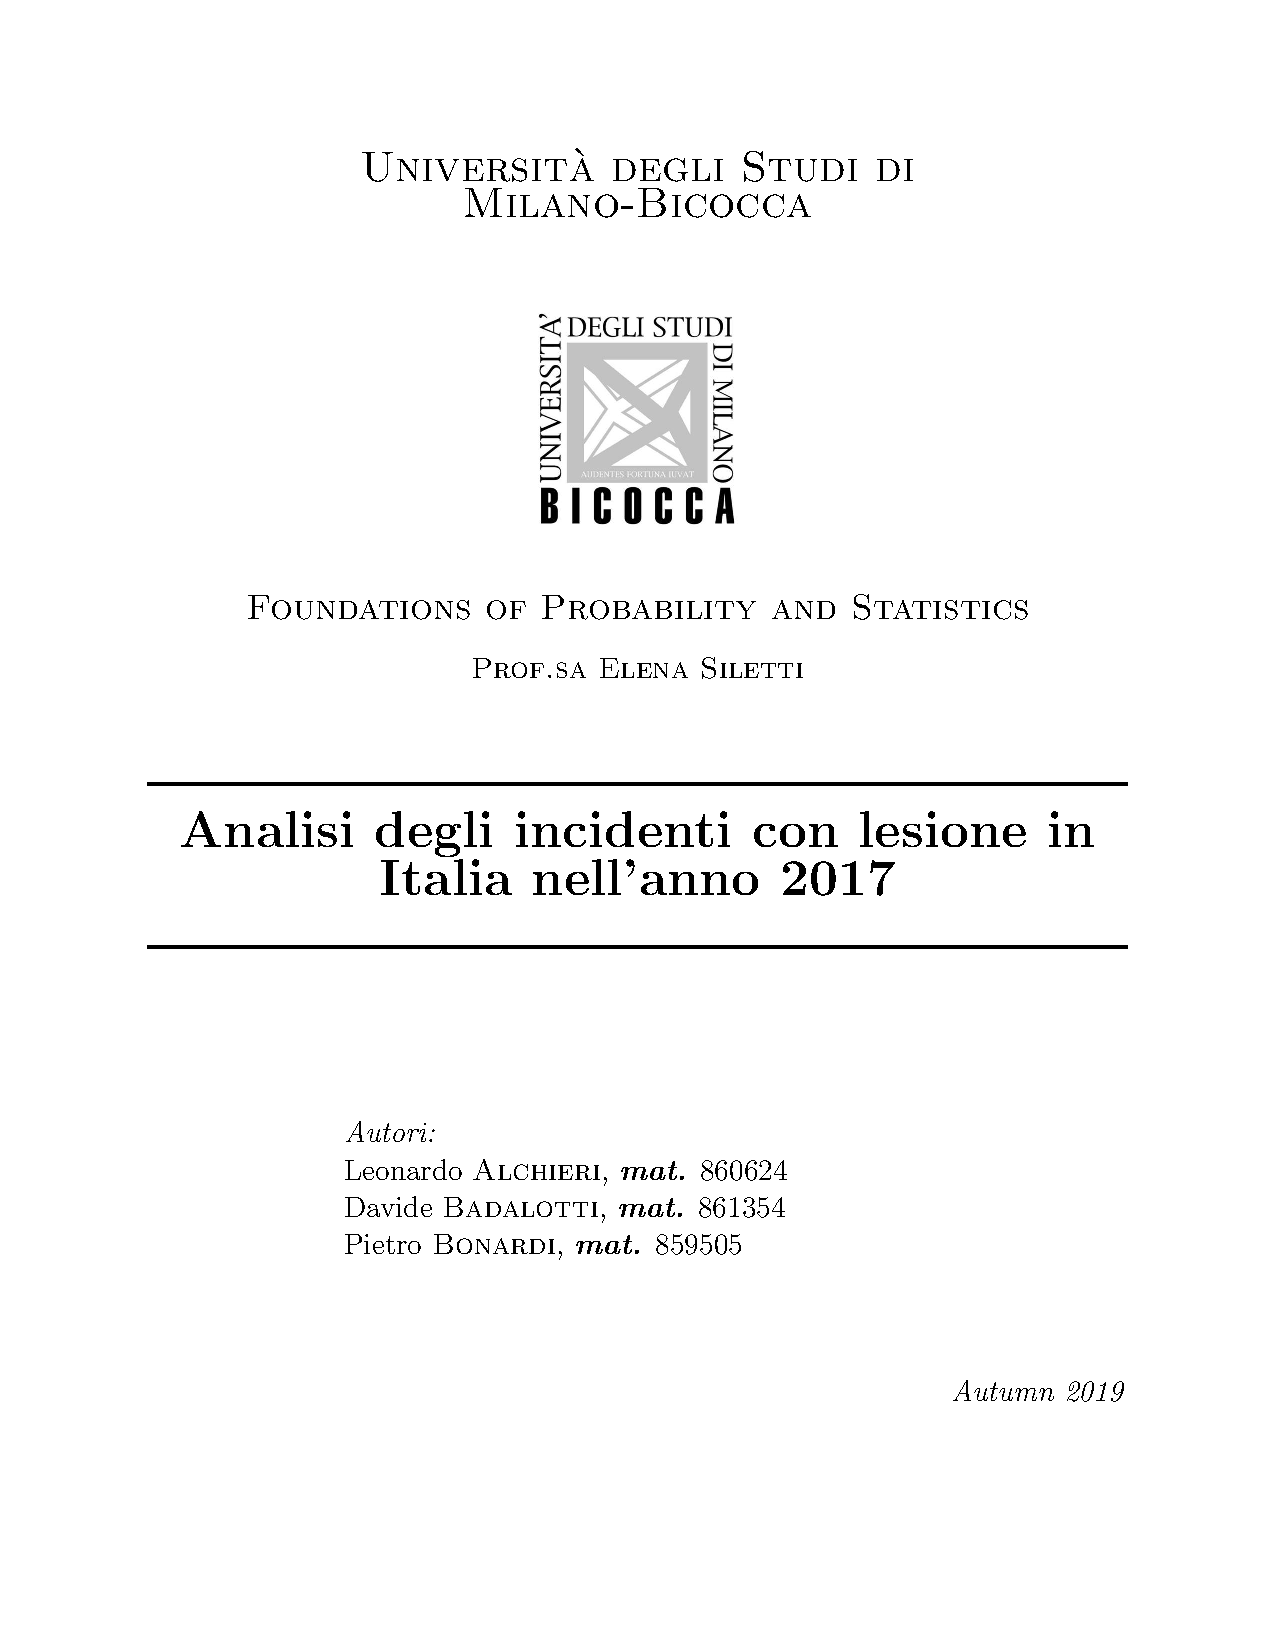
\includepdf{./titlepage/titlepage.pdf}
\end{titlepage}
\blankpage{}
\tableofcontents{}
\clearpage

\section{Introduzione}
	La scelta di analizzare gli incidenti stradali con lesione è quella di voler delineare la pericolosità di guidare un veicolo, diventata oramai un’azione abitudinaria considerando il numero di mezzi in circolazione. I risultati ottenuti sono rivolti ai guidatori e non, in modo da rendere più chiaro a quale rischio ci si “sottopone” ogniqualvolta si è su un autoveicolo. 
	
	\subsection{Spiegazione dei dati}
	In questo progetto abbiamo analizzato statisticamente i dati sugli incidenti  con lesione in Italia nell'anno 2017.
	
	Le fonti dei dati sono:
	\begin{itemize}
		\item Microdati dell'ISTAT su tutta la popolazione di incidenti in Italia nel 2017.
        \item Microdati sulle patenti italiane forniti dal Ministero delle Infrastrutture e dei Trasporti, riferiti alla data 26/05/2017.
        \item Microdati sulle patenti italiane forniti dal Ministero delle Infrastrutture e dei Trasporti, riferiti alla data 26/05/2017.
        \item Dati tabulati dell'ISTAT per la popolazione Italiana per regione, 2019.
	\end{itemize}	
    Tutta l'analisi parte come base dai dati sugli incidenti e usa le altre fonti per eseguire confronti su popolazione. Si noti che, per i casi considerati in questa analisi, si identifica come incidente un qualsiasi evento che coinvolga almeno un veicolo autostradale e comporti la presenza di almeno un ferito e/o morto.
    
    Al fine di eseguire un'analisi campionaria, abbiamo considerato un campione di 20000 incidenti.

\clearpage

\section{Analisi Univariata}
    \subsection{Fascia oraria più critica}
        Quello che vogliamo trovare è l’orario più critico per mettersi alla guida. Da questa analisi, si nota come la concentrazione degli incidenti, come ci si potrebbe aspettare, coincide con le ore di punta. In particolare, gli orari 17 e 18 risultano quelli con più incidenti nel corso della giornata. In Figura \ref{Fig: incidenti_per_ora_orologio} e \ref{Fig: incidenti_per_ora_barrette} sono mostrati gli incidenti per gli orari della giornata.
        
        Precisamente questi due grafici, con granularità di un’ora, mostrano infatti come:
        \begin{itemize}
            \item Le ``17:00",  siano l’orario con frequenza percentuale maggiore di incidenti pari al  7.7\%, nonché la moda. 
            \item Le ``03:00", siano l’orario con frequenza percentuale minore di incidenti pari allo 0.77 \% del totale.
        \end{itemize}
        
        \begin{figure}[t]
        \centering
            \begin{subfigure}{.48\textwidth}
                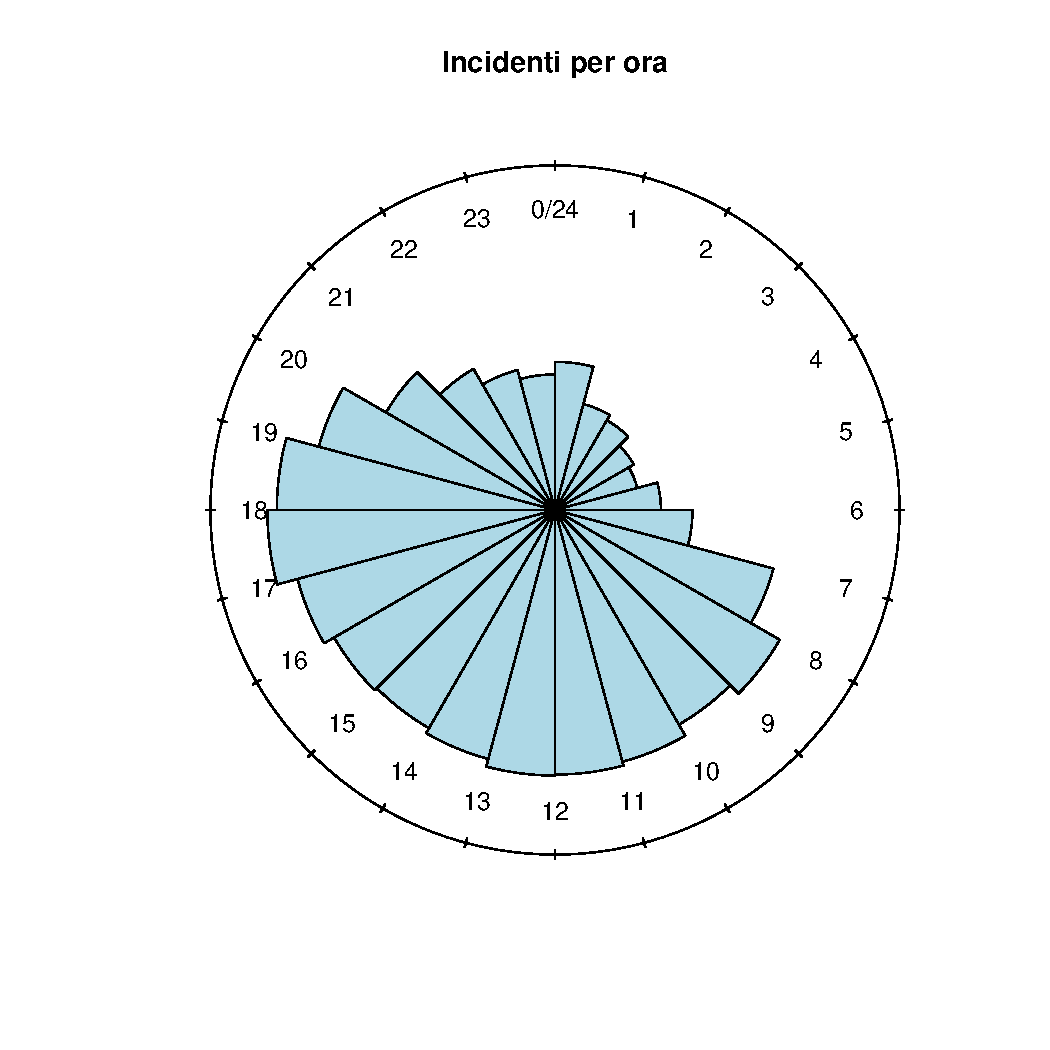
\includegraphics[scale=0.35]{./../results/incidenti_per_ora_orologio.pdf}
                \caption{Grafico a rosa che mostra più chiaramente le frequenze degli incidenti per fascia oraria.}
                \label{Fig: incidenti_per_ora_orologio}
            \end{subfigure}
            \hfill
            \begin{subfigure}{.48\textwidth}
                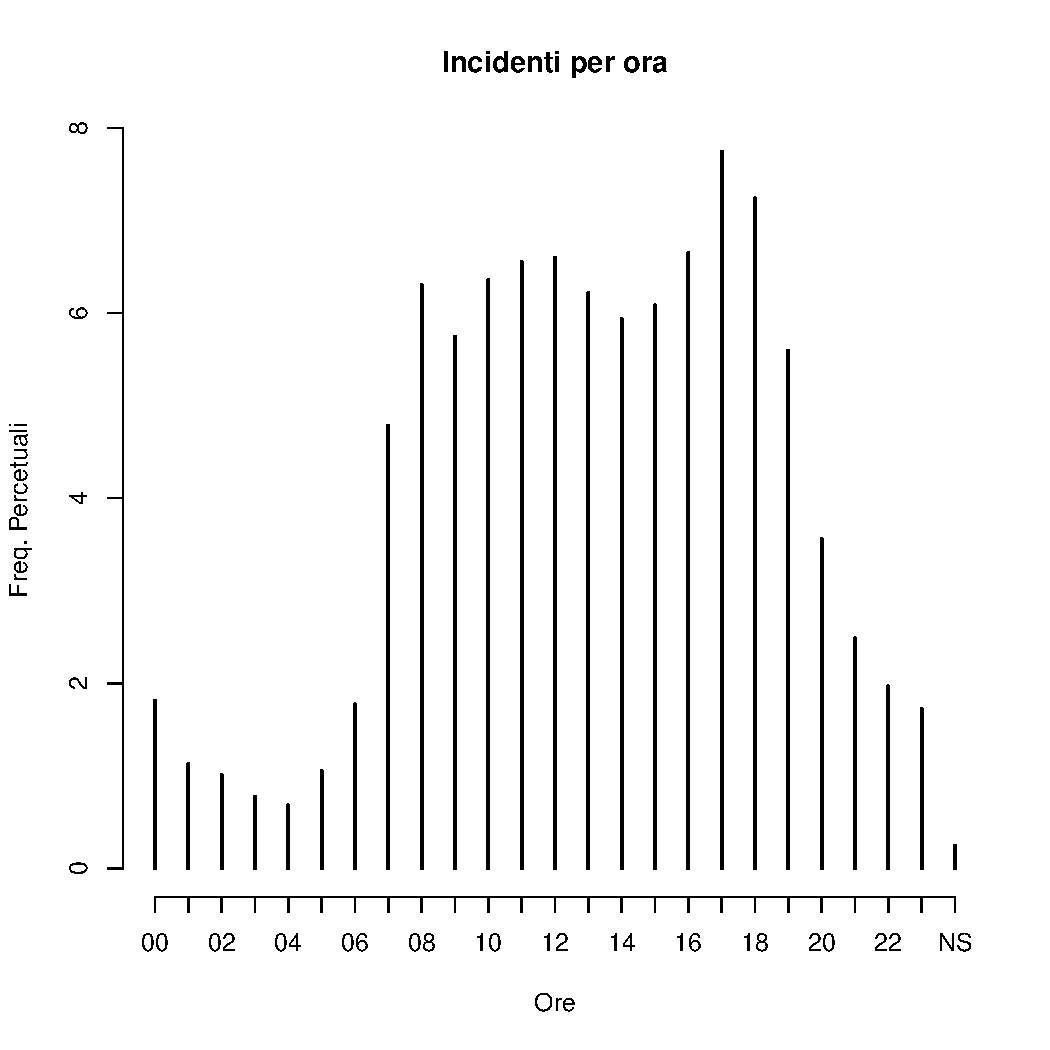
\includegraphics[scale=0.35]{./../results/incidenti_per_ora.pdf}
                \caption{Grafico a bastoncini che specifica per ogni ora la frequenza percentuale di incidenti.}
                \label{Fig: incidenti_per_ora_barrette}
            \end{subfigure}
            \caption{}
        \end{figure}

\clearpage        
    \subsection{L'autostrada con più incidenti}
        Analizziamo gli incidenti nei tratti autostradali, che essi siano denominati con la lettera A (autostrada), R (raccordo) o T (tronco). Purtroppo, per difficoltà di reperibilità, non siamo riusciti a paragonare con la lunghezza dell'autostrada e/o il traffico. Questo fa sì che questa piccola analisi non mostri l'autostrada più pericolosa su cui guidare, ma semplicemente quella in cui sono presenti più incidenti.
        
        \begin{figure}[h!]
            \centering
            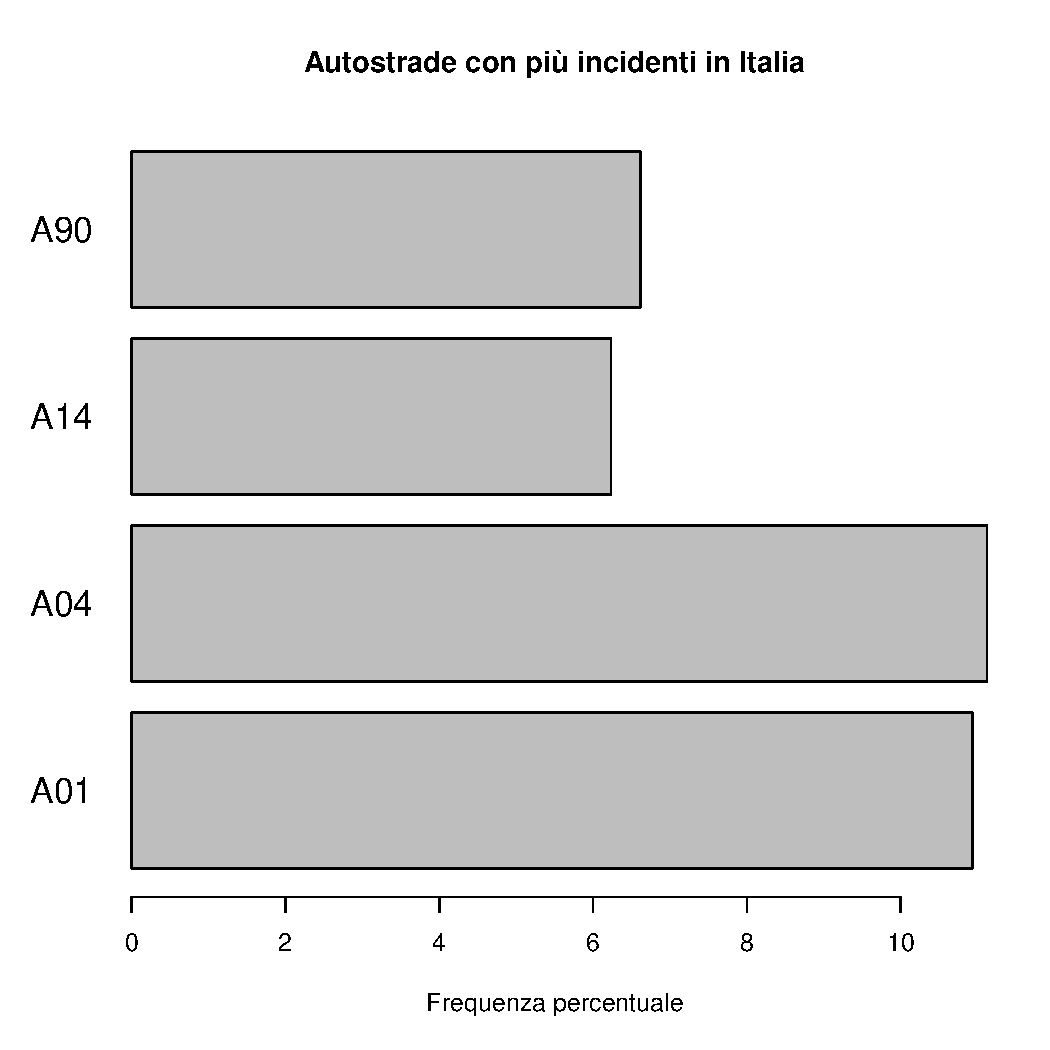
\includegraphics[scale=0.6]{./../results/maggiori_autostrade.pdf}
            \caption{Grafico a barre che specifica la frequenza percentuale delle 4 autostrade con più incidenti.}
            \label{Fig: incidenti_autostrade}
        \end{figure}
        
        L'autostrada con più incidenti in Italia nel 2017 è la A01. 
        
        Purtroppo non siamo riusciti ad ottenere i dati per il traffico sulle diverse autostrade, e quindi rimane limitata nei suoi obiettivi: non siamo in grado di concludere quale sia la più pericolosa.
        
        Rimane comunque il fatto che, qualora una persona decidesse di mettersi alla guida, essere a conoscenza del tratto autostradale con più incidenti in Italia può risultare un'informazione utile.
\clearpage
    \subsection{Le principali aree metropolitane}
        Si sono considerate per principali le città metropolitane di: Torino, Genova, Milano, Roma e Napoli. 
        
        Una prima analisi, senza la considerazione della popolazione, mostra come la città con il maggior numero di incidenti sia Roma (Figura \ref{Fig: citta_metropolitane_tot}). In Figura \ref{Fig: citta_metropolitane_per_abitanti} viene mostrata la stessa analisi, ma pesata sul numero di abitanti.
        
        \begin{figure}[h!]
            \begin{subfigure}{0.48\textwidth}
                \centering
                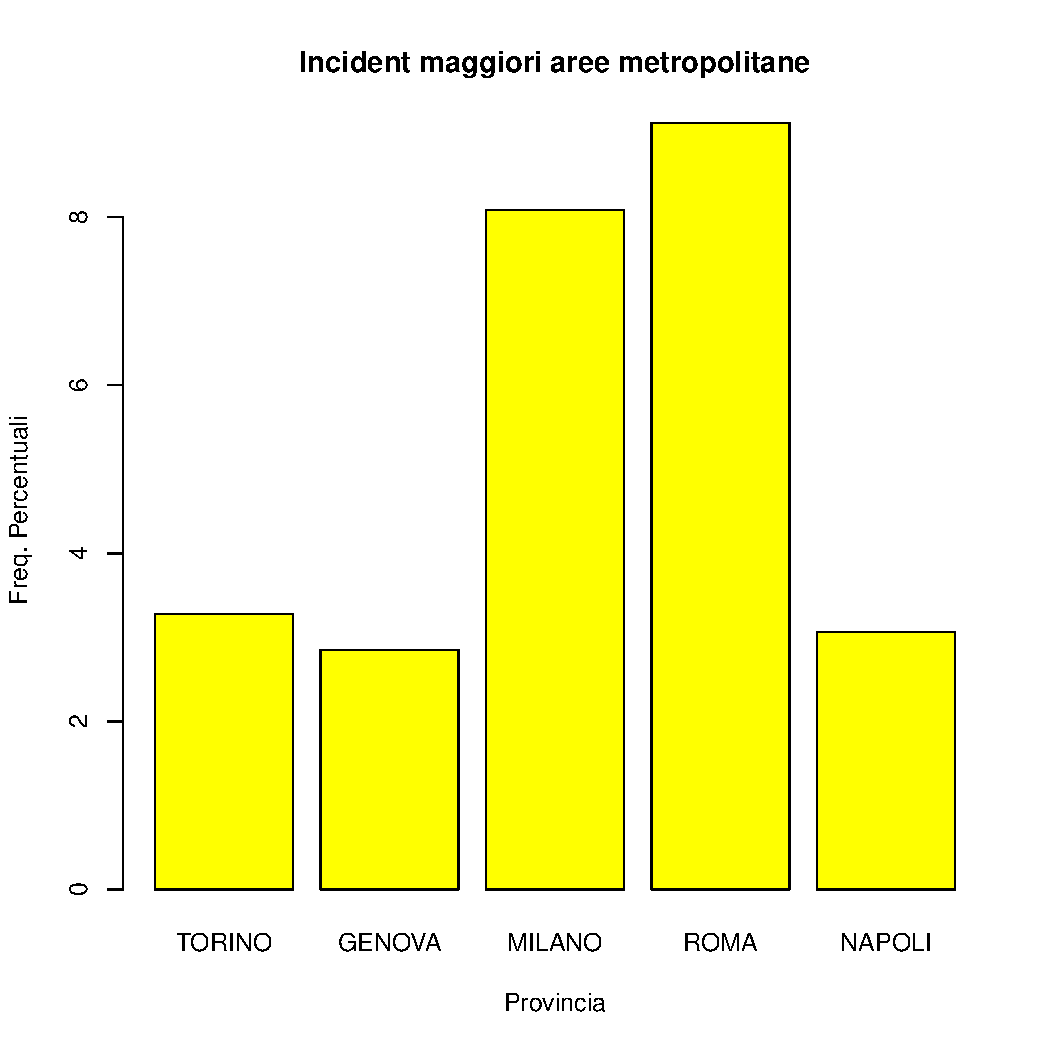
\includegraphics[scale=0.4]{../results/incidenti_maggiori_aree_metropolitane.pdf}
                \caption{Grafico a barre che specifica la frequenza percentuale degli incidenti sulle principali aree metropolitane senza considerare il numero di abitanti.}
                \label{Fig: citta_metropolitane_tot}
            \end{subfigure}
            \hfill
            \begin{subfigure}{0.48\textwidth}
                \centering
                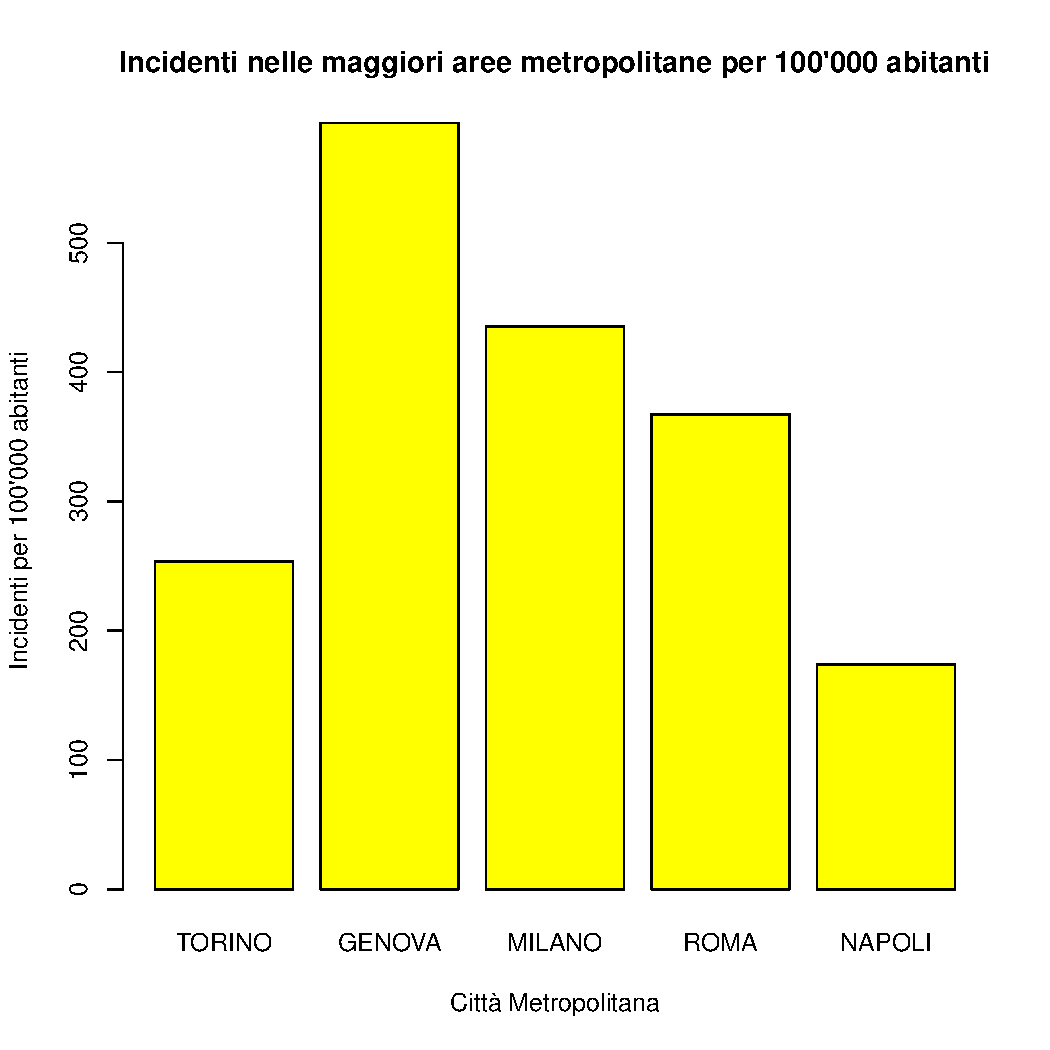
\includegraphics[scale=0.4]{../results/incidenti_per_abitante_aree_metropolinate.pdf}
                \caption{Grafico a barre che specifica la frequenza percentuale degli incidenti sulle principali aree metropolitane pesata sul numero di abitanti di ciascuna. }
                \label{Fig: citta_metropolitane_per_abitanti}
            \end{subfigure}
            \caption{}
        \end{figure}
        
        Sebbene Roma sia la città metropolitana che presenta in totale il maggior numero di incidenti, è Genova la città che, per numero di abitanti, ha più incidenti. In particolare, tra quelle analizzate, Napoli è la città col minor numero di incidenti, sia in assoluto che sugli abitanti.
        
    \subsection{La distribuzione degli incidenti nelle regioni italiane}
    
        Per avere un’indice di pericolosità su ogni regione italiana abbiamo per prima cosa calcolato il numero di incidenti per abitante nelle diverse regioni. 
        
        Il grafico sottostante, Figura \ref{Fig: mappa_incidenti_regioni_per_abitanti}, mostra le frequenze relative per regione. Come si può notare, la Lombardia è la regione con più incidenti per abitante, seguita da Lazio ed Emilia Romagna.
        
        \begin{figure}[h]
            \begin{subfigure}{0.4\textwidth}
                \centering
                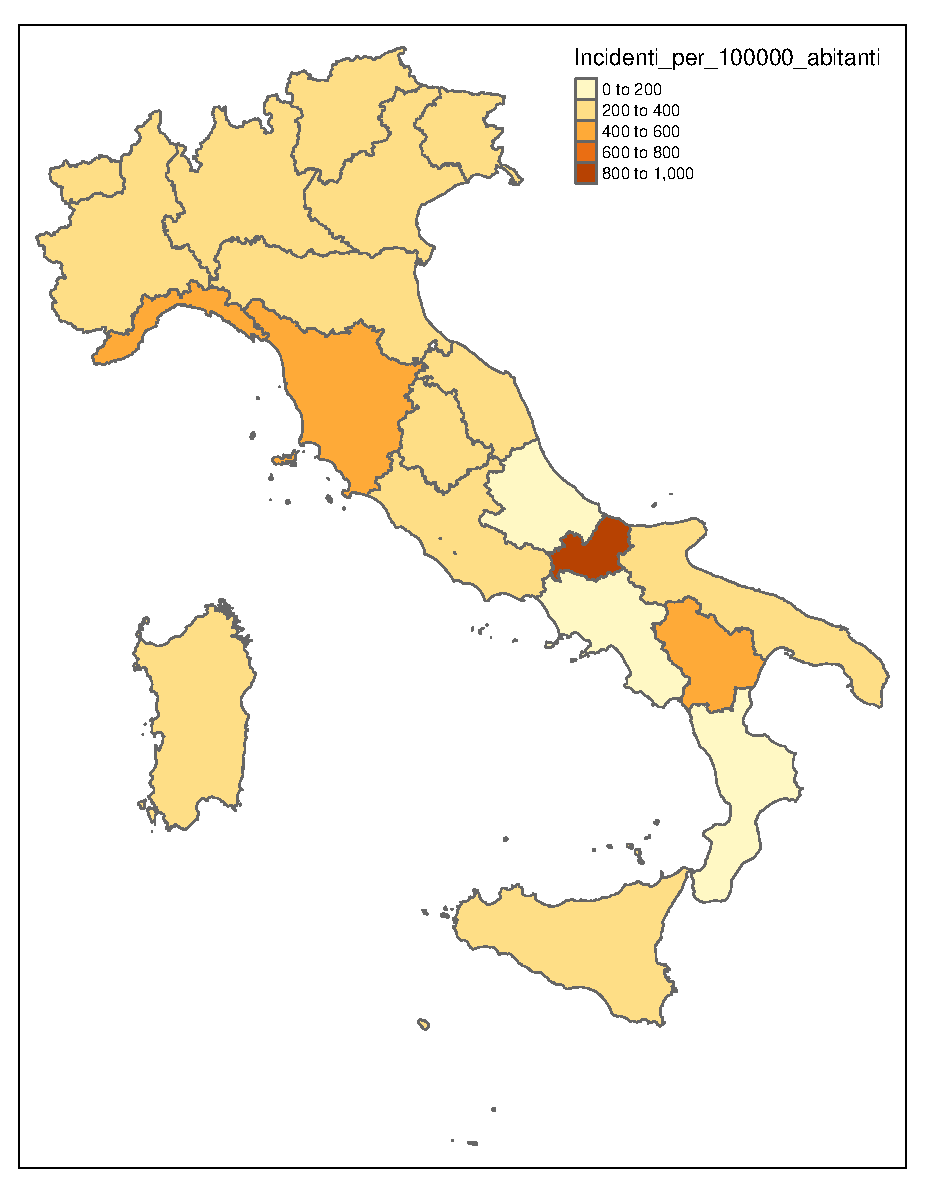
\includegraphics[scale=0.4]{../results/incidenti_per_100000_abitanti.pdf}
                \caption{Cartogramma che mostra le regioni d’Italia con le frequenze relative degli incidenti per abitante.}
                \label{Fig: mappa_incidenti_regioni_per_abitanti}
            \end{subfigure}
            \hfill
            \begin{subfigure}{0.4\textwidth}
                \centering
                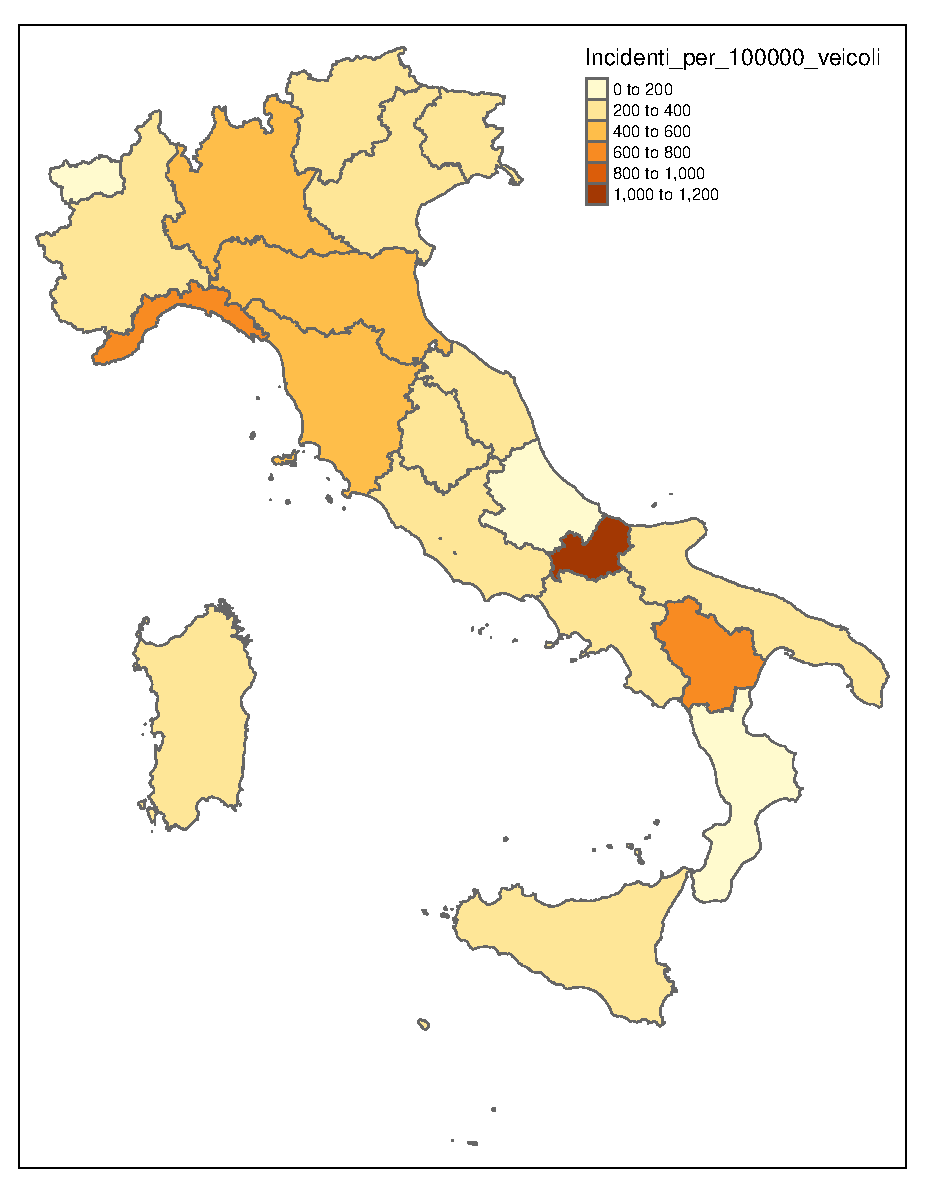
\includegraphics[scale=0.4]{../results/incidenti_per_100000_veicoli.pdf}
                \caption{Cartogramma che mostra le regioni d’Italia con le frequenze relative degli incidenti per abitante.}
                \label{Fig: mappa_incidenti_regioni_per_veicoli}
            \end{subfigure}
            \caption{}
        \end{figure}
        
        In Figura \ref{Fig: mappa_incidenti_regioni_per_veicoli} abbiamo ripetuto il procedimento per il parco veicolare, ovvero per il numero di veicoli in ogni regione. A nostro parere, questo potrebbe risultare essere un indice migliore per valutare la pericolosità di una specifica regione. 
        
        
        
        Come ci si potrebbe aspettare, Lombardia, Emilia Romagna ed Lazio rimangano tra le più rischiose, a cui si aggiungono in ordire Toscana, Abruzzo e Basilicata. Sopra queste risulta però esservi il Molise, il quale è la regione con il maggior numero di incidenti sul parco veicolare.
        
    \subsection{Confronto tra numero di feriti e numero di morti}
    
        Andiamo di seguito a mostrare il numero di morti e feriti per incidente stradale. Per prima cosa, mostriamo un semplice paragone tra feriti e morti per incidenti.
        Si ricordi che i nostri dati sono quelli di incidenti in cui è presente almeno un ferito, per cui non stupisce se vi sia un numero particolarmente alto di feriti per incidenti. Purtroppo, non è possibile avere a disposizione informazioni relative a tutti gli incidenti.
        
        Le Figure \ref{Fig: numero_morti_per_incidente} e \ref{Fig: numero_feriti_per_incidente} mostrano quanti morti o feriti ci sono in ogni incidente stradale. Ovvero, qual è la probabilità che in un incidente vi siano morti o, analogamente, feriti.
        
        \begin{figure}[h!]
            \begin{subfigure}{0.48\textwidth}
                \centering
                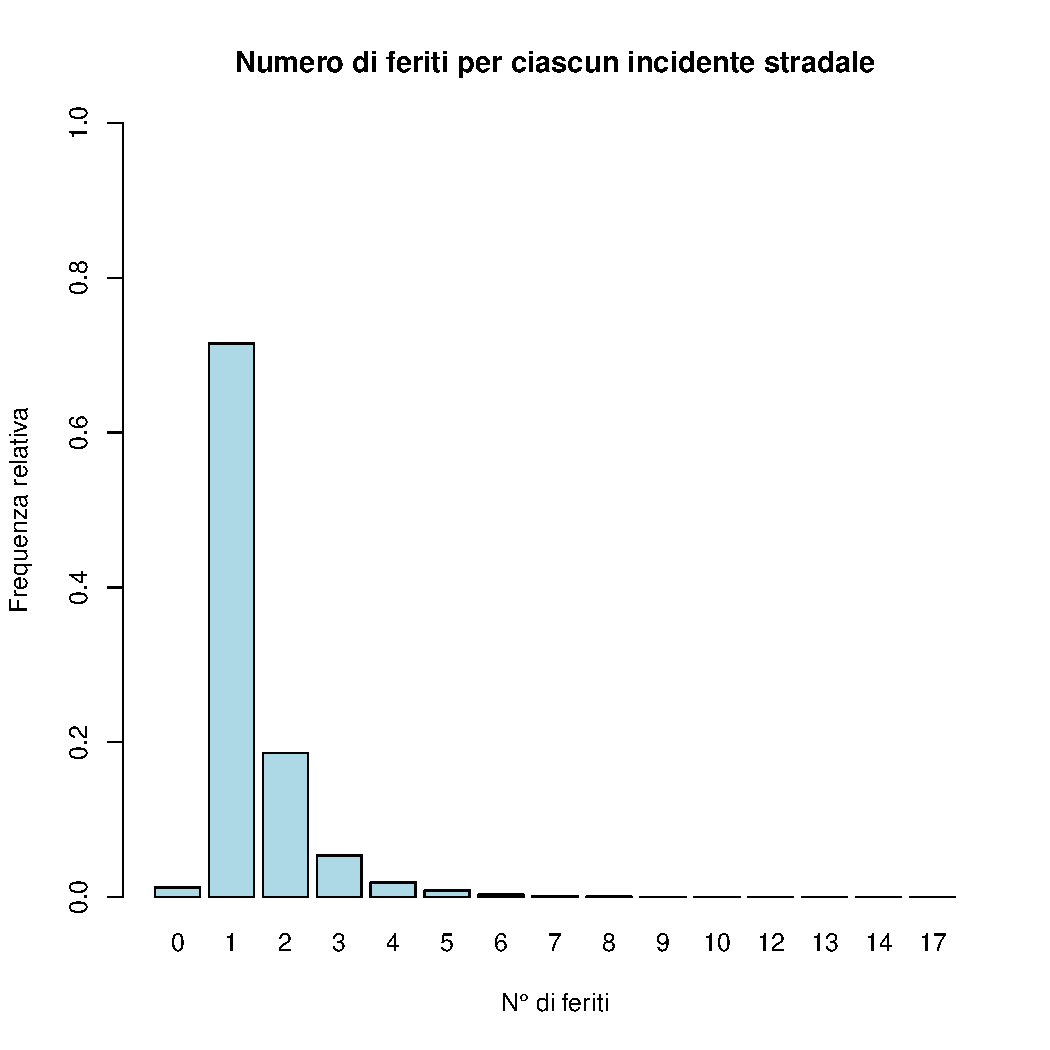
\includegraphics[scale=0.4]{../results/numero_feriti_per_incidente.pdf}
                \caption{Grafico a barre che mostra le frequenze relative del numero di feriti in un incidente.}
                \label{Fig: numero_morti_per_incidente}
            \end{subfigure}
            \hfill
            \begin{subfigure}{0.48\textwidth}
                \centering
                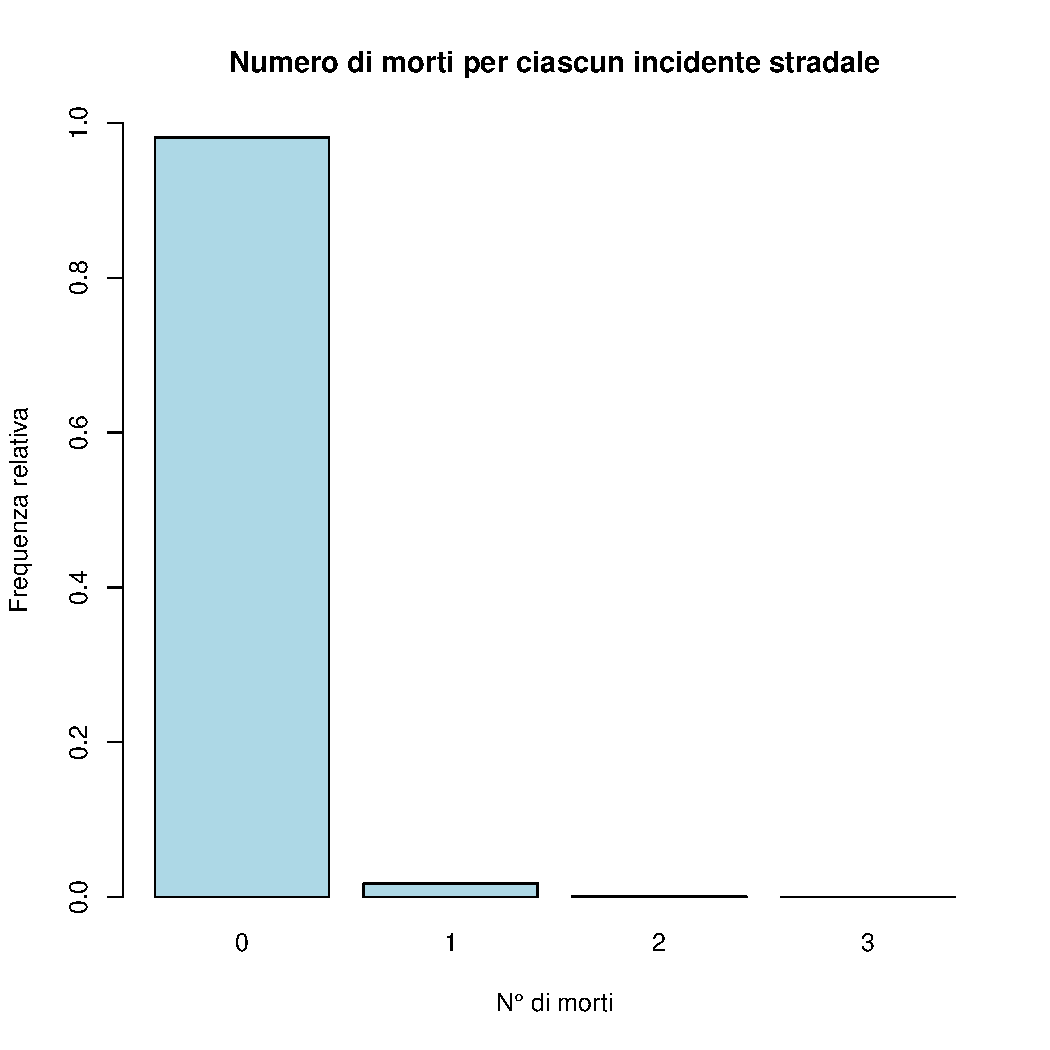
\includegraphics[scale=0.4]{../results/numero_morti_per_incidente.pdf}
                \caption{Grafico a barre che mostra le frequenze relative del numero di morti in un incidente.}
                \label{Fig: numero_feriti_per_incidente}
            \end{subfigure}
            \caption{}
        \end{figure}
        \begin{figure}[h!]
            \centering
            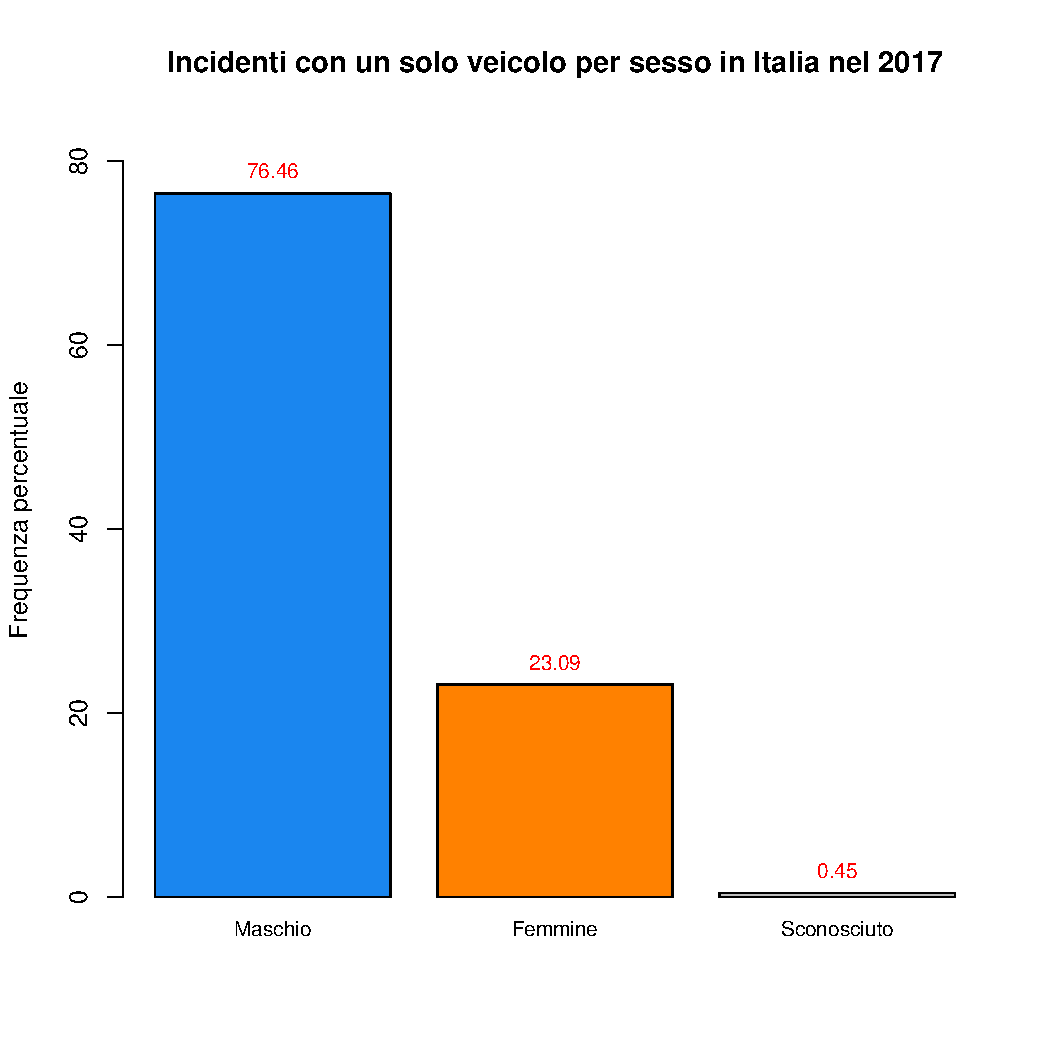
\includegraphics[scale=0.5]{../results/incidenti_per_sesso.pdf}
            \caption{Grafico a barre che mostra le frequenze percentuali degli incidente per genere.}
            \label{Fig: sesso_incidenti}
        \end{figure}
        
    \subsection{Genere guidatore più ``pericoloso" in incidenti con un solo veicolo}

        
        Siamo andati ad analizzare la distribuzione dei sessi negli incidenti in cui è coinvolto un solo veicolo. Ovvero ci siamo posti l'obiettivo di rispondere alla domanda: 
        \begin{quote}
        Chi tra uomini e donne tende a commettere più incidenti da solo?
        \end{quote}
        
        Si noti come questa analisi non rimandi con precisione quale tra i due sessi sia effettivamente più un pericolo, ma solamente comunque quale tra i due tenda a commettere più incidenti da solo.
        
        Il grafico in Figura \ref{Fig: sesso_incidenti} è molto significativo: mostra infatti come vi siano molti più uomini che fanno incidenti da soli rispetto alle donne. Non tiene però conto del fatto che vi siano più uomini che donne alla guida. Abbiamo quindi eseguito un'analisi più dettagliata, nella quale siamo andati a considerare anche la percentuale di patenti in Italia per i rispettivi sessi.
        
        
        
        Come indicato all'inizio, siamo andati a prendere i microdati relativi alle patenti fornite dal Ministero delle Infrastrutture e dei Trasporti per il 2017. In Figura \ref{Fig: tot_patenti} si mostra la distribuzione delle patenti in Italia.
        \begin{figure}[h]
        \centering
            \begin{subfigure}{0.5\textwidth}
                
                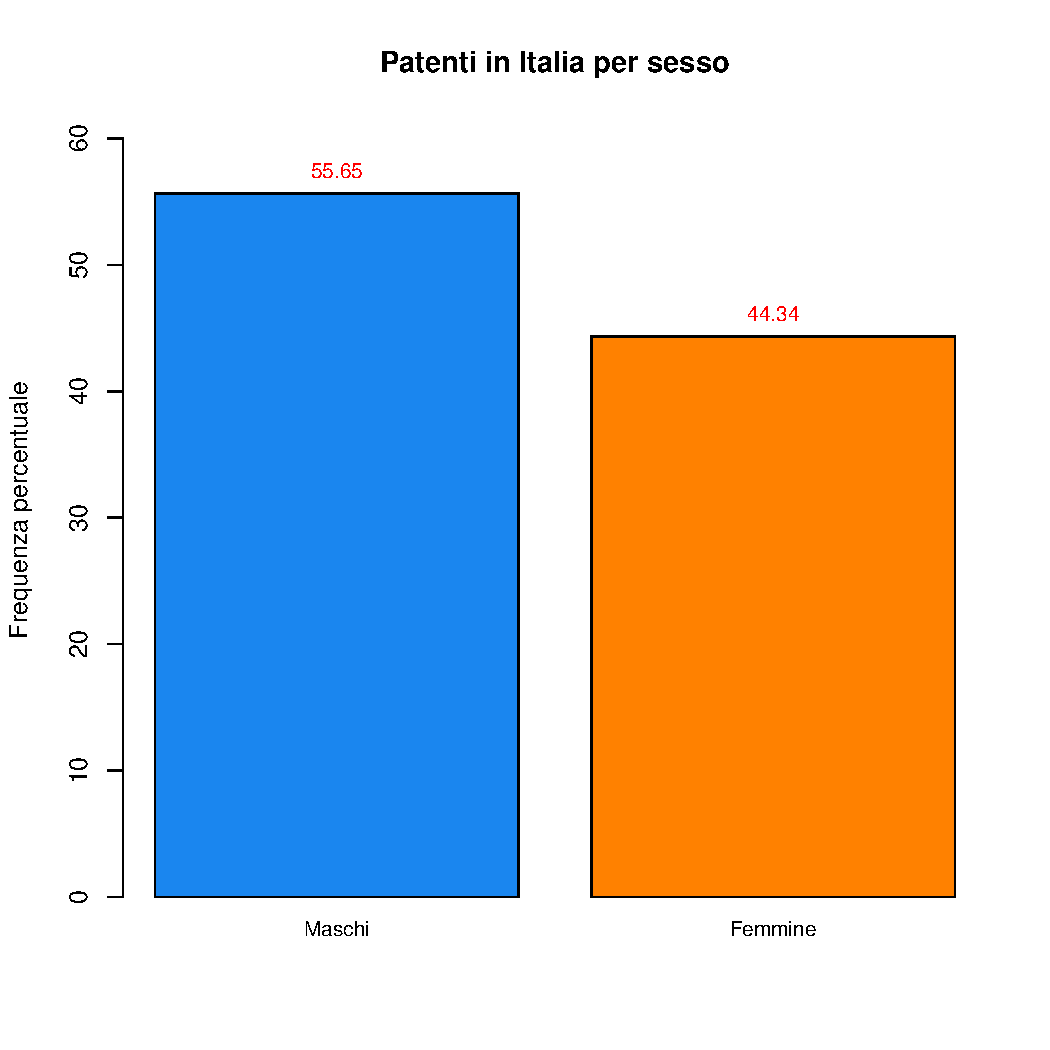
\includegraphics[scale=0.5]{../results/patenti_per_sesso.pdf}
                \caption{Grafico a barre che mostra le frequenze percentuali delle patenti per genere.}
                \label{Fig: tot_patenti}
            \end{subfigure}
            
            \begin{subfigure}{0.5\textwidth}
                
                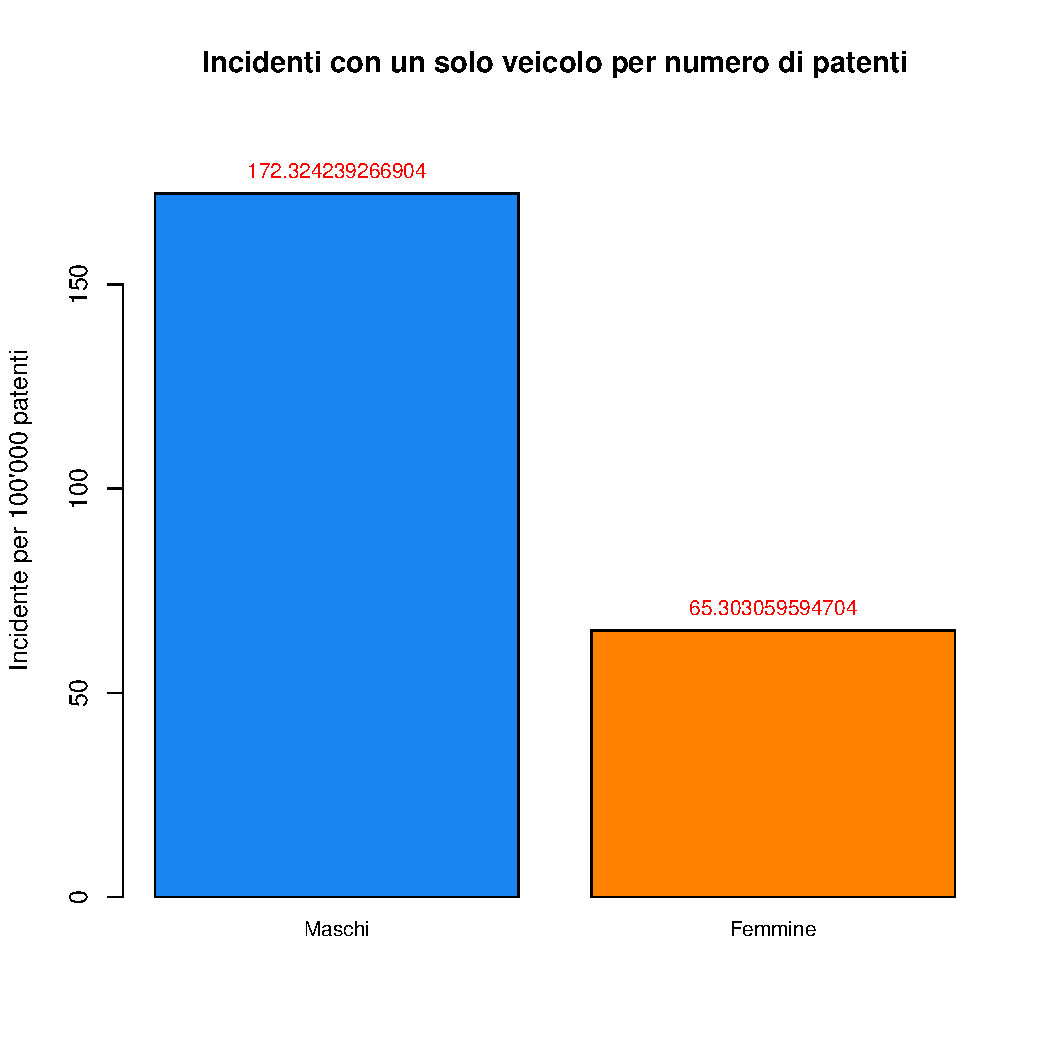
\includegraphics[scale=0.5]{../results/incidenti_per_sesso_per_patenti.pdf}
                \caption{Grafico a barre che mostra il numero di incidenti per 100’000 patenti. }
                \label{Fig: incidenti_per_sesso_patenti}
            \end{subfigure}
            \caption{}
        \end{figure}
        
        Dividendo il numero di incidenti dei due sessi per il rispettivo numero di patenti, abbiamo ottenuto la distribuzione degli incidenti per numero di patenti per entrambi i sessi, come mostrato in Figura \ref{Fig: incidenti_per_sesso_patenti}.
        
        È importante notare come questi dati non permettano di capire la probabilità che un maschio (o viceversa una femmina) commetta un incidente. È però possibile mostrare quanto sia più probabile che un maschio commetta un incidente da solo rispetto a una femmina. Abbiamo trovato che gli uomini sono il $148.65\%$ più probabili di causare un incidente con un solo veicolo coinvolto rispetto alle donne.
\clearpage

\section{Analisi dell’impatto di alcuni fattori di rischio sul numero medio di morti e feriti per incidente stradale}
    
    In questa sezione prendiamo in considerazione il numero di morti e feriti per singolo incidente stradale e li analizziamo in un funzione dei seguenti fattori:
    \begin{itemize}
        \item Trimestre in cui avviene l’incidente
        \item Ora del giorno in cui avviene l’incidente
        \item Tipo di fondo stradale su cui avviene l’incidente
        \item Tipo di strada su cui avviene l’incidente
        \item Qualità della pavimentazione stradale su cui avviene l’incidente
    \end{itemize}
    Per ciascun fattore analizzato, la logica con cui viene condotta l’indagine è pressoché identica, perciò verrà illustrata nel dettaglio solo per il primo caso visto.
    
    \subsection{Analisi trimestrale}\label{Sec: analisi_trimestrale}
        Di seguito, in Figura \ref{Fig: vittime_incidenti_trimestre}, vengono riportati i grafici che illustrano il numero medio di feriti e vittime per incidente stradale suddivisi nei vari trimestri.
        
        \begin{figure}[h]
            \begin{subfigure}{0.4\textwidth}
                \centering
                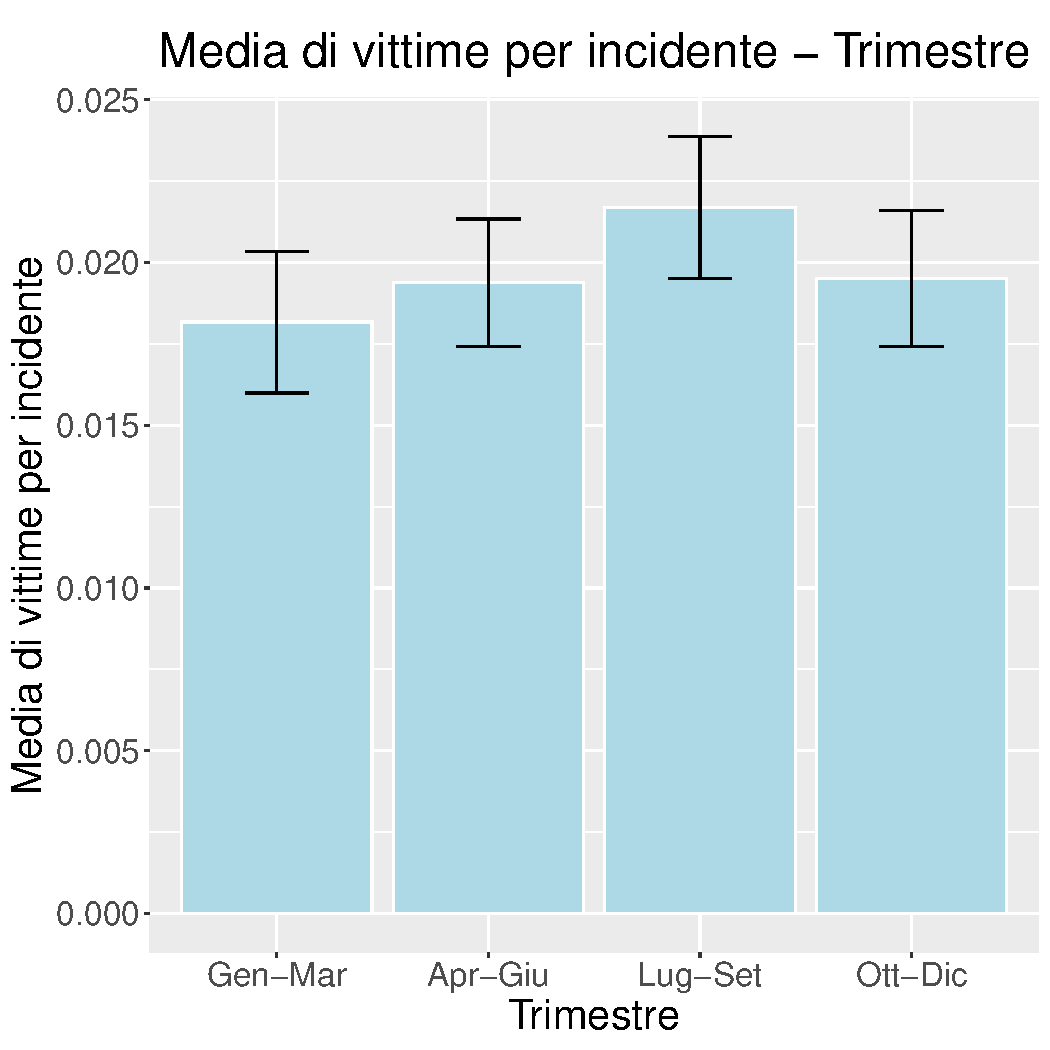
\includegraphics[scale=0.4]{../results/media_morti_per_incidente_trimestre.pdf}
            \end{subfigure}
            \hfill
            \begin{subfigure}{0.4\textwidth}
                \centering
                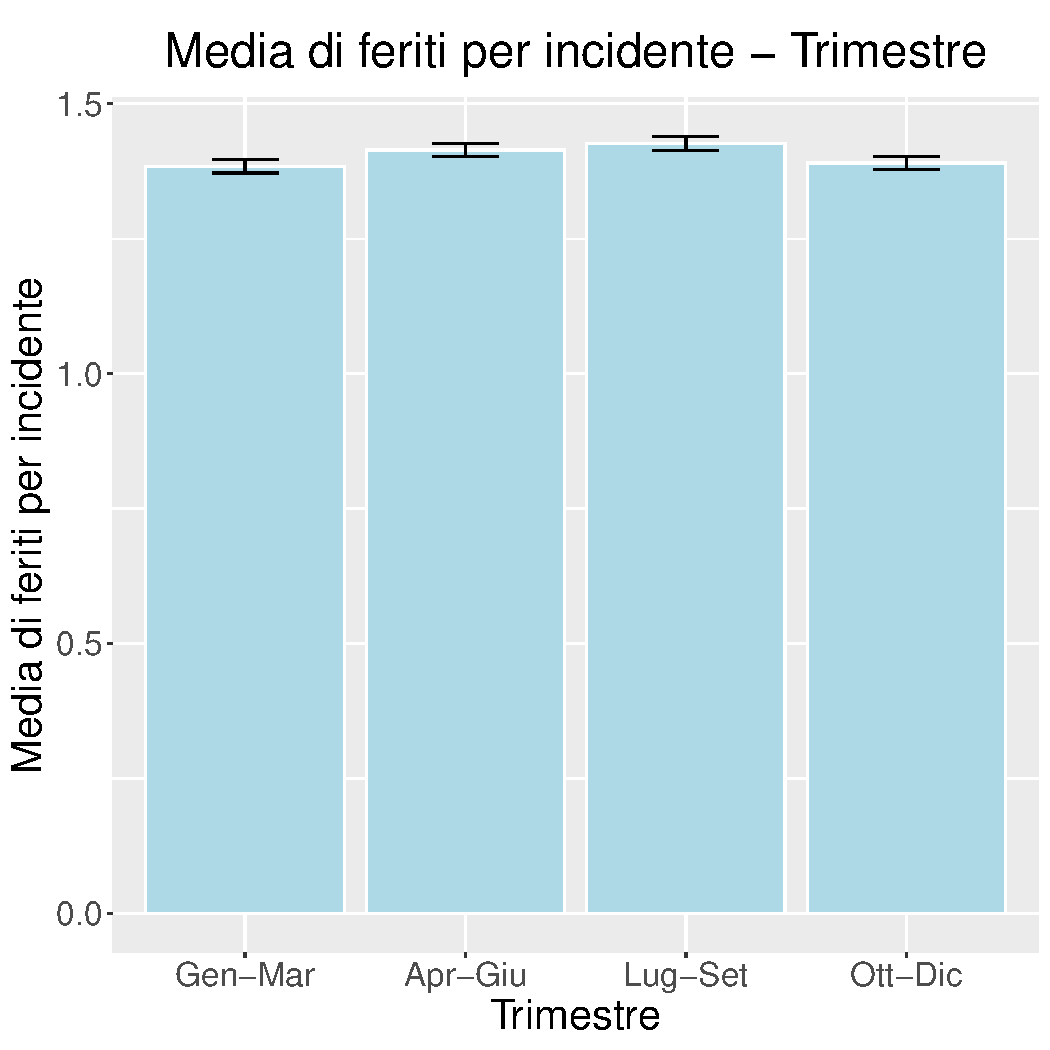
\includegraphics[scale=0.4]{../results/media_feriti_per_incidente_trimestre.pdf}
            \end{subfigure}
            \caption{Due grafici a barre che mostrano, rispettivamente, la media di feriti e vittime per incidente nei diversi trimetri dell’anno.}
            \label{Fig: vittime_incidenti_trimestre}
        \end{figure}
    
        L’obiettivo dello studio è quello di effettuare dei test di ipotesi per confrontare il numero medio di morti o feriti nei vari trimestri. A tal fine, possiamo ipotizzare che il numero di vittime e di feriti per ciascun incidente sia rappresentabile da variabili casuali discrete, indipendenti e aventi stessa distribuzione di probabilità. 
        Sappiamo, inoltre, che, in funzione del teorema del limite centrale, la quantità:
        \[
            Z = \frac {\bar X - \mu}{s / {\sqrt n } }
        \]
        tende ad una distribuzione normale standardizzata. Dove con $\bar X $ si indica il numero medio di vittime/feriti per ciascun incidente, con $\mu$ il valor medio delle due quantità appena citate, con $s$ le loro deviazioni standard e con $n$ la numerosità del campione.
        
        Ovviamente, disponendo solamente dei dati relativi al campione, e non conoscendo il valor medio  e la deviazione standard , siamo costretti ad utilizzare le loro stime campionarie. 
        
        Riassumendo le nostre ipotesi, quindi:
        \begin{itemize}
            \item $X$, numero di vittime/feriti per singolo incidente stradale, NON tende ad una distribuzione normale.
            \item $\sigma$ non è nota ma stimata dal campione.
	    \item $n$ è sufficientemente grande perché si possa considerare $Z \sim N(0, 1)$ in virtù del teorema del limite centrale
        \end{itemize}
        
        Prendiamo quindi, in considerazione, i dati relativi ai feriti nei vari trimestri. Conduciamo un primo test d’ipotesi, così strutturato:
        \begin{itemize}
            \item $H_0$: il numero medio di feriti per incidente stradale nel trimestre Aprile-Giugno è uguale al numero medio di feriti per incidente relativo al trimestre Luglio-Settembre.
            \item $H_1$: il numero medio di feriti per incidente stradale nel trimestre Aprile-Giugno è diverso dal numero medio di feriti per incidente relativo al trimestre Luglio-Settembre. 
            \item Confidence level: 99\%
        \end{itemize}
        Si calcola quindi $Z_{test}$, definita come:
        \[
            Z_{test} = \frac { (\bar X _1 - \bar X_2) - ( \mu_1 - \mu_2)} { \sqrt{var(\bar X_1 - \bar X_2)}}
        \]
        Dove ovviamente $\mu_1 - \mu_2 = 0 $. Al valore di $Z_{test}$ si abbina il p-value corrispondente, definito come:
        \[
            p-value = 2P(Z > | Z_{test}|)
        \]
        ed estrapolato da una distribuzione normale.

        Si ottiene in questo caso:
        \[
            Z_{test} = 1.145
        \]
        \[
            p-value = 0.2522
        \]
        Possiamo, quindi, affermare che \textbf{il test non è statisticamente significativo} e che non disponiamo di sufficienti dati per rifiutare l’ipotesi nulla.
        \smallskip
        Con la stessa logica consideriamo il numero medio di vittime nei vari trimestri. Conduciamo un primo test d’ipotesi, così strutturato:
        \begin{itemize}
            \item $H_0$: il numero medio di vittime per incidente stradale nel trimestre Aprile-Giugno è uguale alla media relativa al trimestre Luglio-Settembre.
            \item $H_1$: il numero medio di vittime per incidente stradale nel trimestre Aprile-Giugno è diverso dalla media relativa al trimestre Luglio-Settembre.
            \item Livello di significatività: 99\%
        \end{itemize}
        Si ottiene in questo caso:
        \[
            Z_{test} = 0.675
        \]
        \[
            p-value = 0.49968
        \]
        Come nel caso precedente, \textbf{il test non è statisticamente significativo} e non disponiamo di dati a sufficienza per rifiutare l’ipotesi nulla.

        Attraverso le stesse ipotesi e la stessa logica, analizziamo anche l’impatto di altri fattori sulle grandezze appena esposte.
        
        Si noti bene che, non potendo effettuare test d’ipotesi multipli (che richiederebbero metodi di correzione del p-value), ci siamo limitati a confrontare, per ciascun fattore (trimestre, ora, fondo stradale ecc..), solo due modalità, che abbiamo ritenuto più significative. 

    \subsection{Analisi di morti e feriti per ore del giorno}
        Riportiamo di seguito, in Figura \ref{Fig: incidenti_per_ora_morti_feriti}, il grafico che illustra il numero medio di feriti per incidente stradale nelle varie ore della giornata, con le relative deviazioni standard della media. 
        
        \begin{figure}[h]
            \begin{subfigure}{0.4\textwidth}
                \centering
                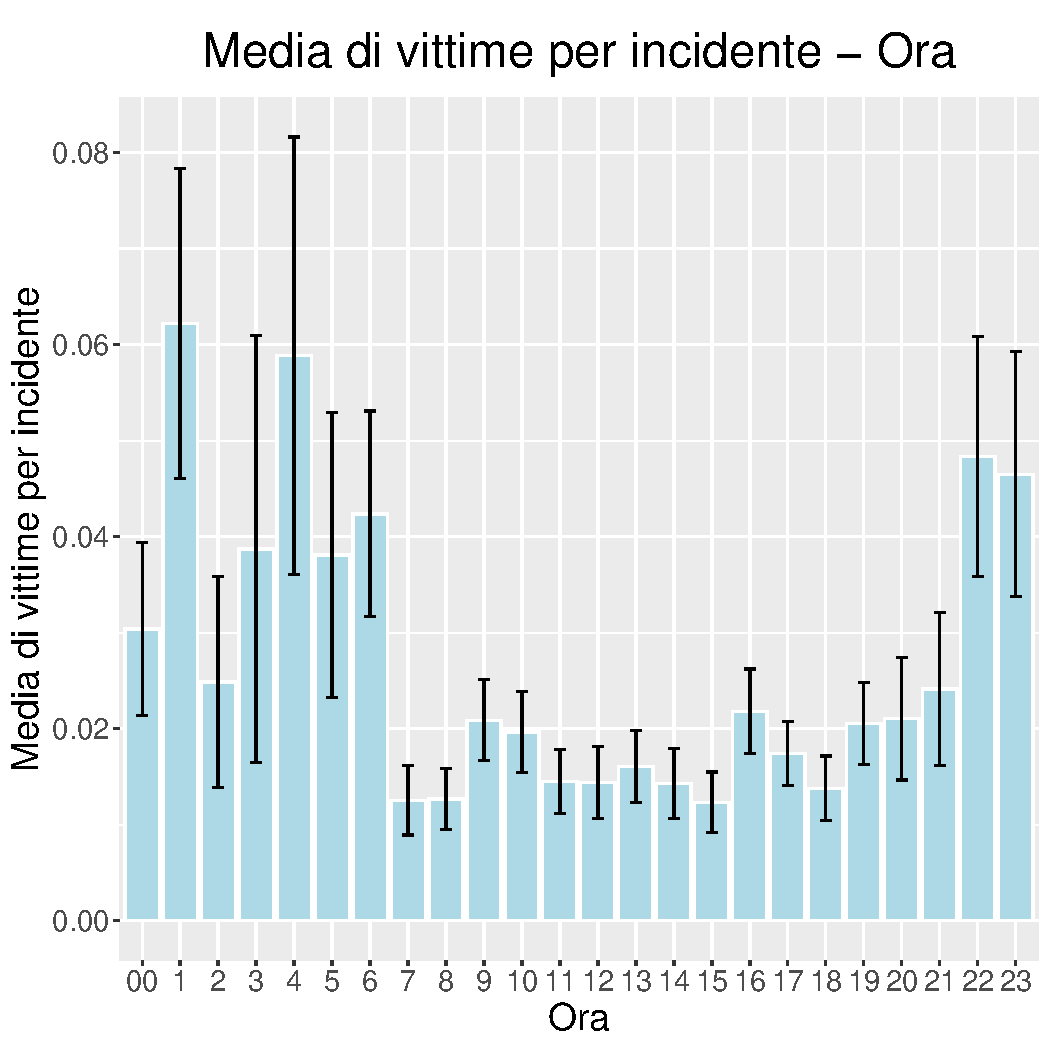
\includegraphics[scale=0.4]{../results/media_morti_per_incidente_ora.pdf}
            \end{subfigure}
            \hfill
            \begin{subfigure}{0.4\textwidth}
                \centering
                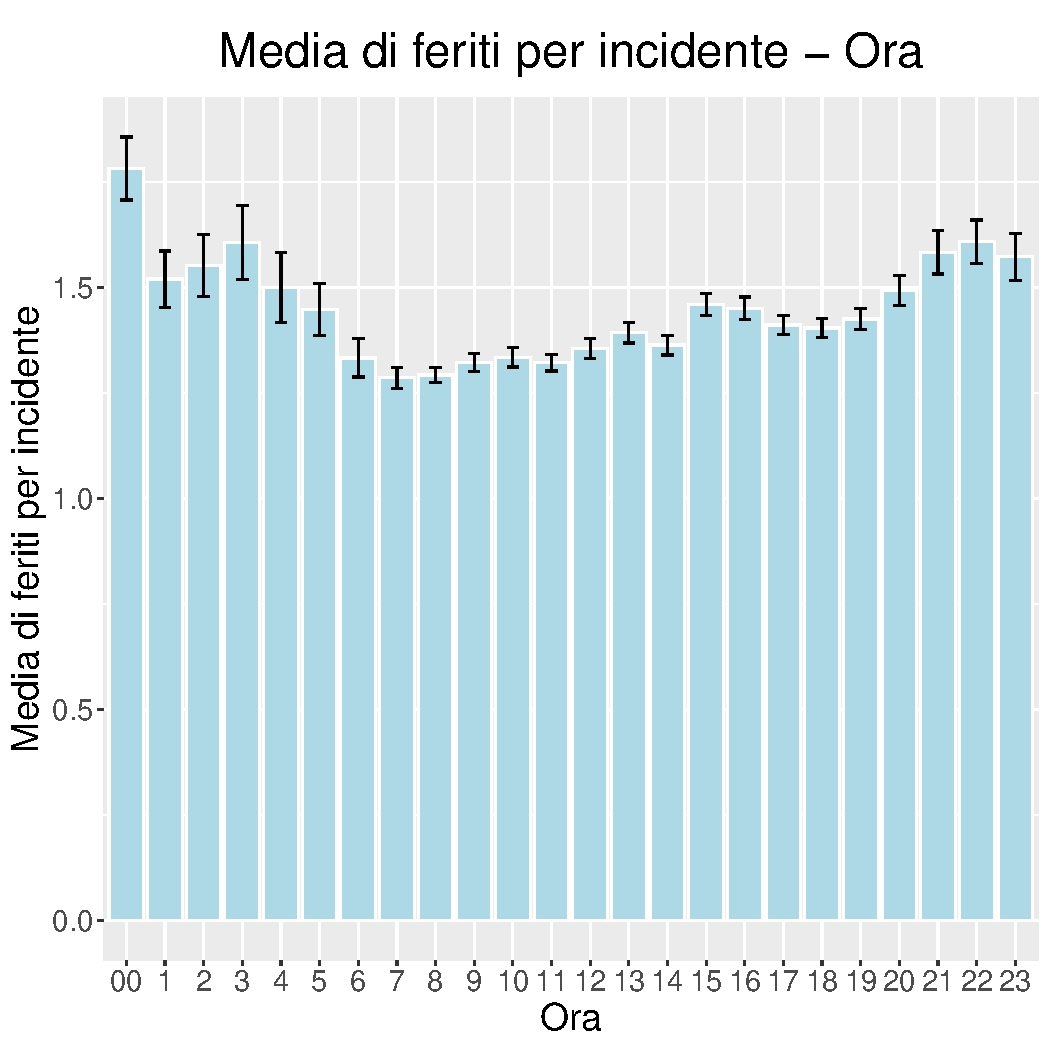
\includegraphics[scale=0.4]{../results/media_feriti_per_incidente_ora.pdf}
            \end{subfigure}
            \caption{Due grafici a barre che mostrano, rispettivamente, la media di feriti e vittime per incidente nelle diverse ore della giornata.}
            \label{Fig: incidenti_per_ora_morti_feriti}
        \end{figure}
        Sempre seguendo la logica della sezione precedente, effettuiamo un test d’ipotesi così strutturato:
        \begin{itemize}
            \item $H_0$: il numero medio di feriti per incidente stradale all’ora 1 è uguale al tasso di feriti per incidente stradale alle ore 3.
            \item $H_1$: il numero medio di feriti per incidente stradale all’ora 1 è diverso dal tasso di feriti per incidente stradale alle ore 3.
            \item Confidence level: 99\%.
        \end{itemize}
        Abbiamo ottenuto per i feriti:
        \[
            Z_{test} = 3.487
        \]
        \[
            p-value = 0.00048
        \]
        \textbf{Il test è statisticamente significativo}. Pertanto si rifiuta l’ipotesi nulla.
        
        Sempre in Figura \ref{Fig: incidenti_per_ora_morti_feriti} si può vedere il grafico che illustra il numero medio di vittime per incidente stradale suddiviso nelle varie ore del giorno, con le relative deviazioni standard della media.
        
         Il test d’ipotesi effettuato è il seguente:
         \begin{itemize}
             \item $H_0$: il numero medio di vittime per incidente stradale alle ore 4 è uguale al tasso di vittime per incidente stradale alle ore 8.
            \item $H_1$: il numero medio di vittime per incidente stradale alle ore 4 è diverso dal tasso di vittime per incidente stradale alle ore 8.
            \item Confidence level: 99\%.
         \end{itemize}
        I risultati sono:
        \[
            Z = 1.983
        \]
        \[
            p-value = 0.0508
        \]
        Il test non è statisticamente significativo. Non si può rifiutare l’ipotesi nulla.
        
    \subsection{Analisi di morti e feriti per fondo stradale}
        Si riporta di seguito, in Figura \ref{Fig: fondo_stradale_morti_feriti}, il grafico che mostra il numero medio di feriti per incidente stradale condizionatamente al tipo di fondo stradale, con le relative deviazioni standard della media.
        \begin{figure}[h]
            \begin{subfigure}{0.4\textwidth}
                \centering
                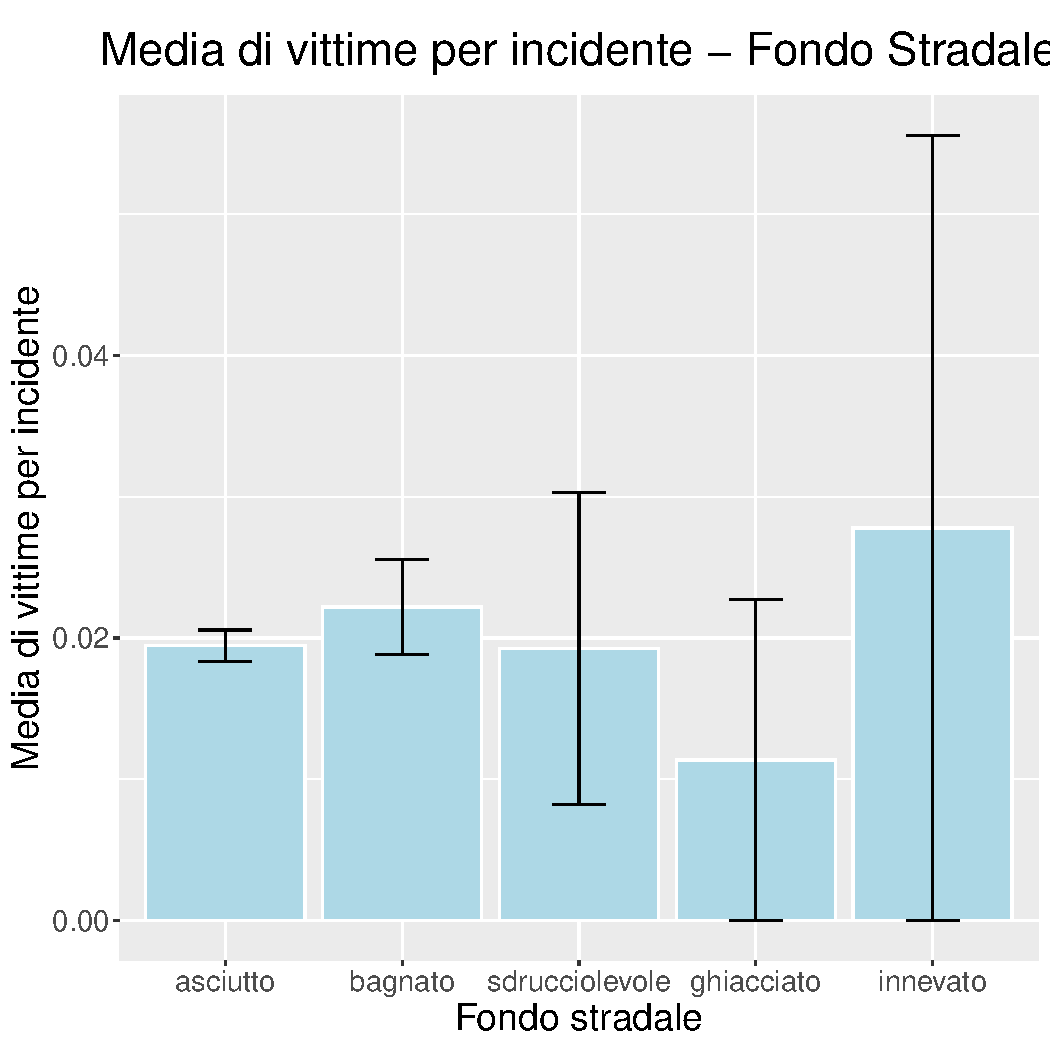
\includegraphics[scale=0.4]{../results/media_morti_per_incidente_fondo.pdf}
            \end{subfigure}
            \hfill
            \begin{subfigure}{0.4\textwidth}
                \centering
                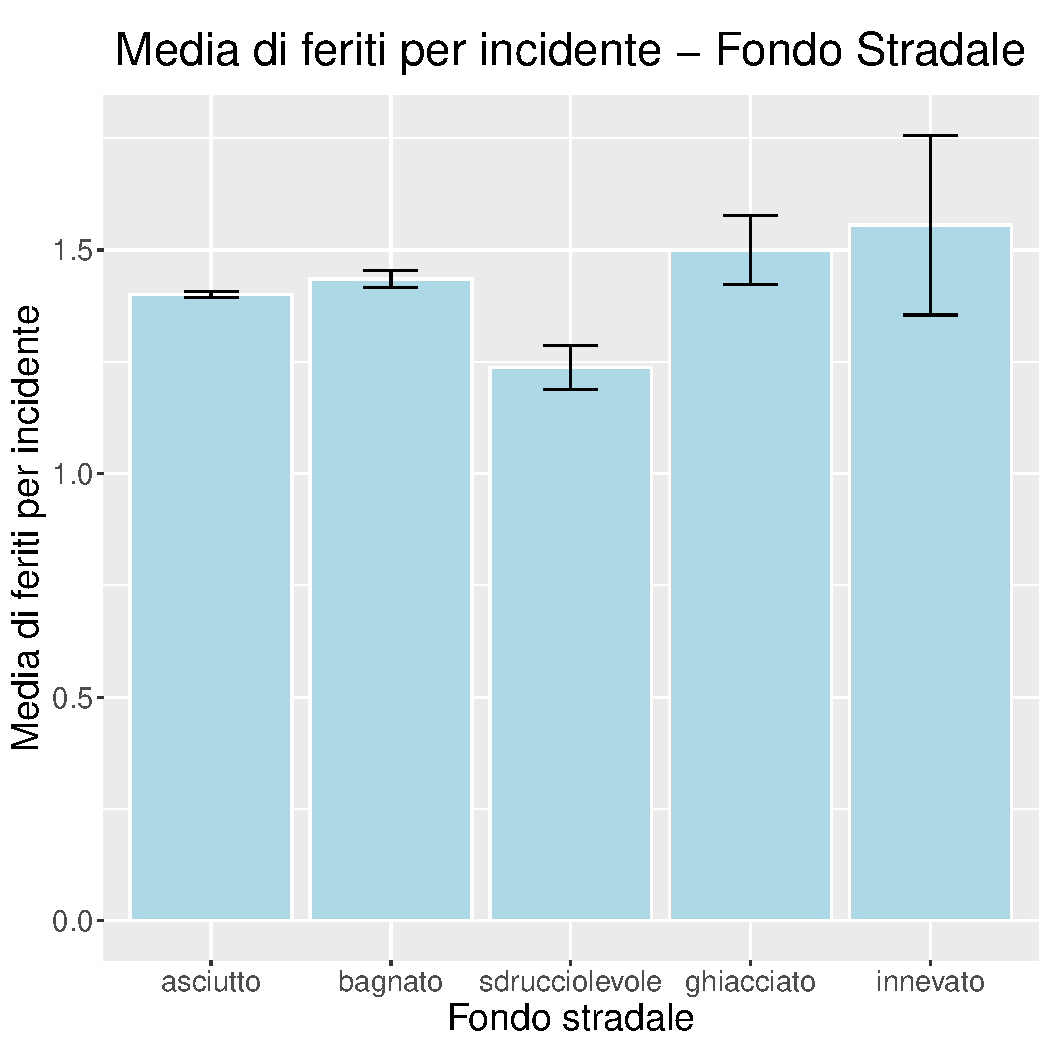
\includegraphics[scale=0.4]{../results/media_feriti_per_incidente_fondo.pdf}
            \end{subfigure}
            \caption{Due grafici a barre che mostrano, rispettivamente, la media di feriti e vittime per incidente nelle diverse ore della giornata.}
            \label{Fig: fondo_stradale_morti_feriti}
        \end{figure}
        Il test condotto riguarda il confronto fra i feriti su fondo sdrucciolevole e asciutto:
        \begin{itemize}
            \item $H_0$: il numero medio di feriti per incidente stradale su fondo asciutto è uguale al tasso di feriti per incidente stradale su fondo sdrucciolevole.
            \item $H_1$: il numero medio di feriti per incidente stradale su fondo asciutto è diverso dal tasso di feriti per incidente stradale su fondo sdrucciolevole
            \item Confidence level: 99\%.
        \end{itemize}
        Per i feriti, i risultati ottenuti sono:
        \[
            Z_{test} = 4.25
        \]
        \[
            p-value = 2\cdot10 ^ {-4}
        \]
        \textbf{Il test è statisticamente significativo}. Si rifiuta l’ipotesi nulla.
        
        Sempre in Figura \ref{Fig: fondo_stradale_morti_feriti} si può vedere il grafico che mostra il numero medio di vittime per incidente stradale condizionatamente al tipo di fondo stradale, con le relative deviazioni standard della media.
        
        Il test condotto è il seguente:
        \begin{itemize}
            \item $H_0$: il numero medio di vittime per incidente stradale su fondo asciutto è uguale al tasso di vittime per incidente stradale su fondo ghiacciato.
            \item $H_1$: il numero medio di vittime per incidente stradale su fondo asciutto è diverso dal tasso di vittime per incidente stradale su fondo ghiacciato.
            \item Confidence level: 99\%.
        \end{itemize}
        In questo caso, i risultati sono:
        \[
            Z_{test} = 1.156
        \]
        \[
            p-value = 0.24768
        \]
        \textbf{Il test non è statisticamente significativo}. Non siamo in grado di rifiutare l’ipotesi nulla.
        
    \subsection{Analisi di morti e feriti per tipo di strada}
        Si riporta, in Figura \ref{Fig: feriti_morti_tipo_strada}, il grafico che illustra il numero medio di feriti per incidente stradale condizionatamente al tipo di strada, con le relative deviazioni standard della media.
        \begin{figure}[h]
            \begin{subfigure}{0.4\textwidth}
                \centering
                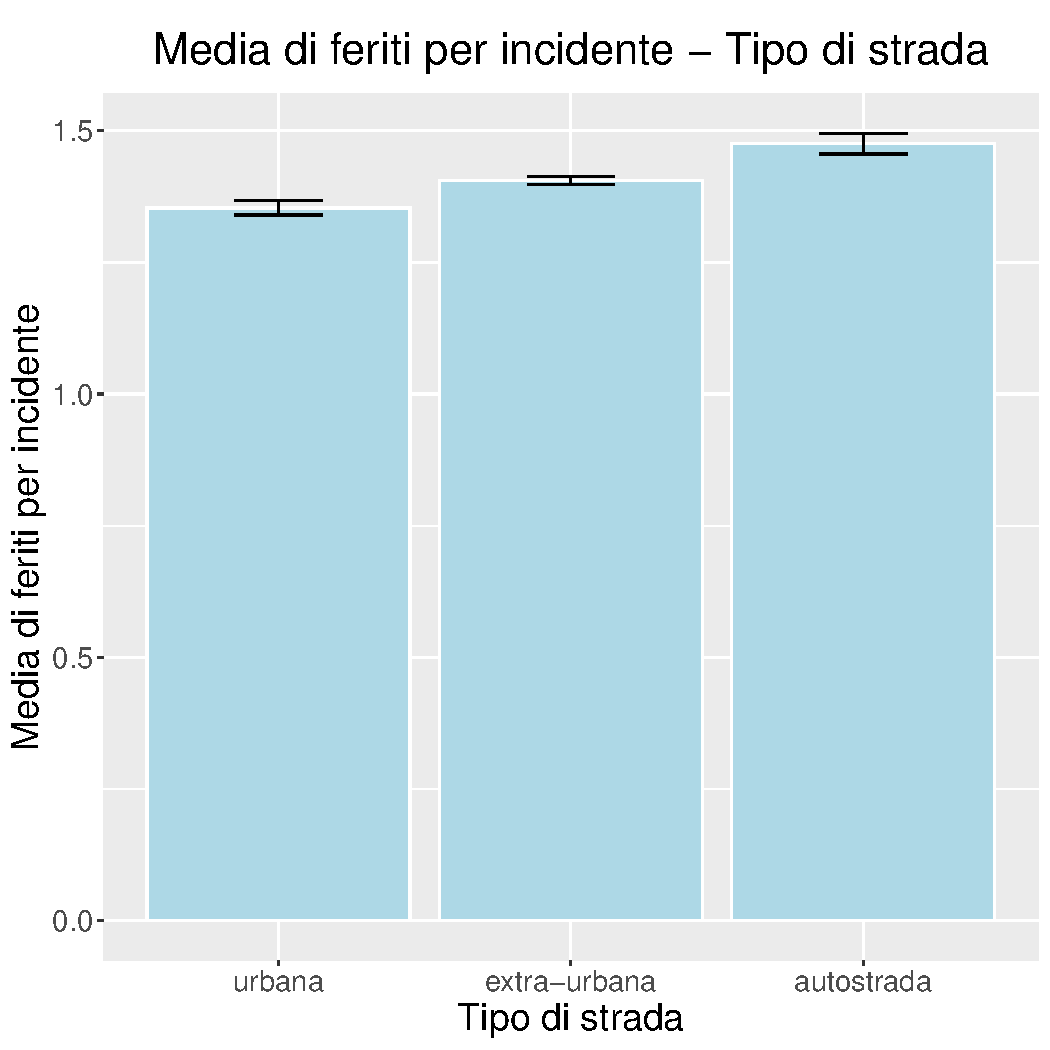
\includegraphics[scale=0.4]{../results/media_feriti_per_incidente_tipo_strada.pdf}
            \end{subfigure}
            \hfill
            \begin{subfigure}{0.4\textwidth}
                \centering
                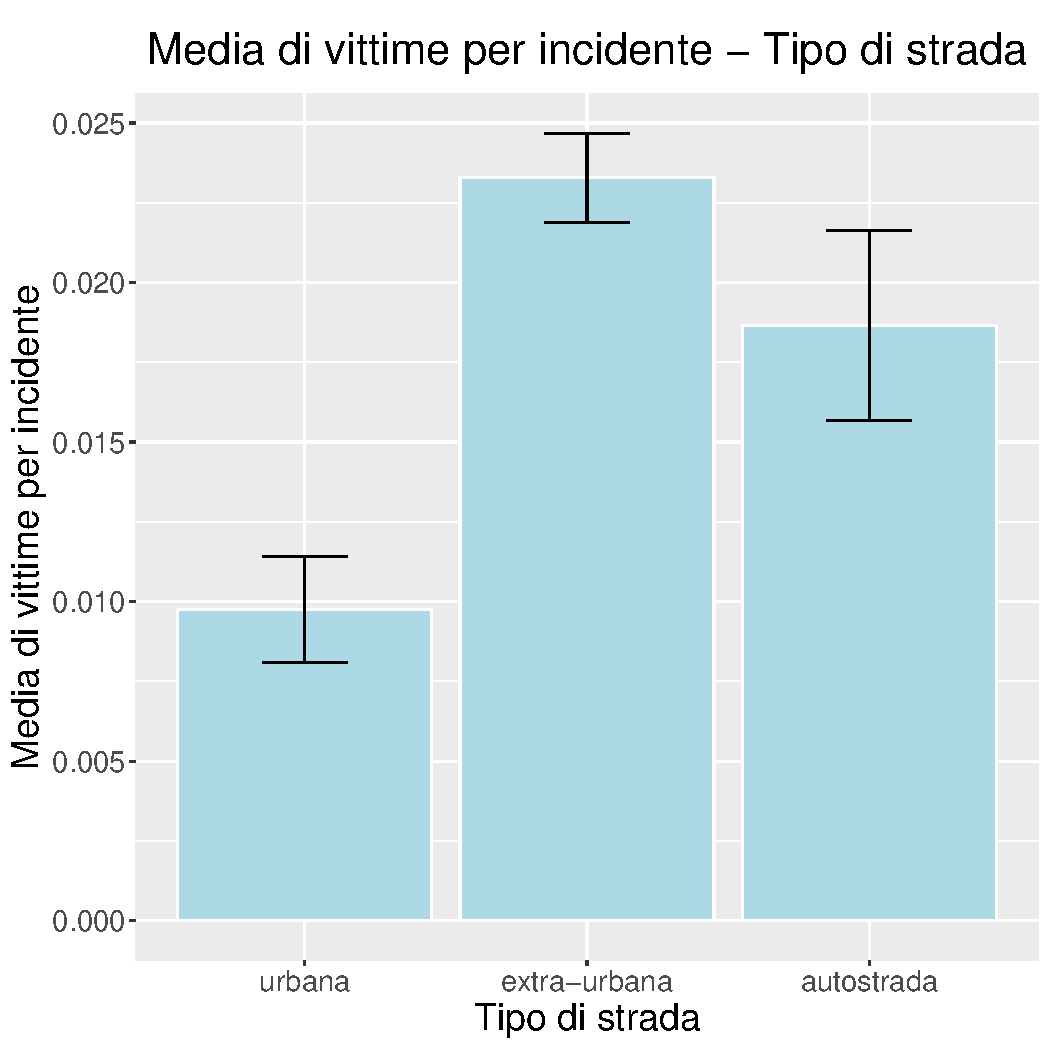
\includegraphics[scale=0.4]{../results/media_morti_per_incidente_tipo_strada.pdf}
            \end{subfigure}
            \caption{Grafici a barre con il numero medio e la deviazione standard di feriti e morti per i diversi tipi di strada.}
            \label{Fig: feriti_morti_tipo_strada}
        \end{figure}        
        Nel test vengono confrontati i feriti per incidenti urbani e autostradali:
        \begin{itemize}
            \item $H_0$: il numero medio di feriti per incidente stradale negli incidenti su strade urbane è uguale al numero di feriti per incidente su autostrade.
            \item $H_1$: il numero medio di feriti per incidente stradale negli incidenti su strade urbane è diverso dal numero di feriti per incidente su autostrade.
            \item Confidence level: 99\%.
        \end{itemize}
        Si è ottenuto:
        \[
            Z_{test} = 13.987
        \]
        \[
            p-value \simeq 0
        \]
        \textbf{Il test è statisticamente significativo}. Si rifiuta l’ipotesi nulla.
        
        Sempre in Figura \ref{Fig: feriti_morti_tipo_strada}, il grafico che illustra il numero medio di vittime per incidente stradale condizionatamente al tipo di strada con le relative deviazioni standard della media.
        
        Il test confronta, come in precedenza, il tasso di morti per incidente stradale su strada urbana e su autostrada.
        \begin{itemize}
            \item $H_0$: il numero medio di vittime per incidente stradale negli incidenti su strade urbane è uguale al numero di vittime per incidente su autostrade.
            \item $H_1$:  il numero medio di vittime per incidente stradale negli incidenti su strade urbane è diverso dal numero di vittime per incidente su autostrade.
            \item Confidence level: 99\%.
        \end{itemize}
        Il risultato ottenuto è:
        \[
            Z_{test} = 1.591
        \]
        \[
            p-value = 0.1116
        \]
        Il test non è statisticamente significativo. Non possiamo rifiutare l’ipotesi nulla.
        
    \subsection{Analisi di morti e feriti per tipo di pavimentazione}
    
        Si riporta nel seguente grafico, Figura \ref{Fig: morti_feriti_pavimentazione}, il numero medio di feriti per incidente stradale al variare del tipo di pavimentazione, con le relative deviazioni standard della media.
        
        \begin{figure}[h]
            \begin{subfigure}{0.4\textwidth}
                \centering
                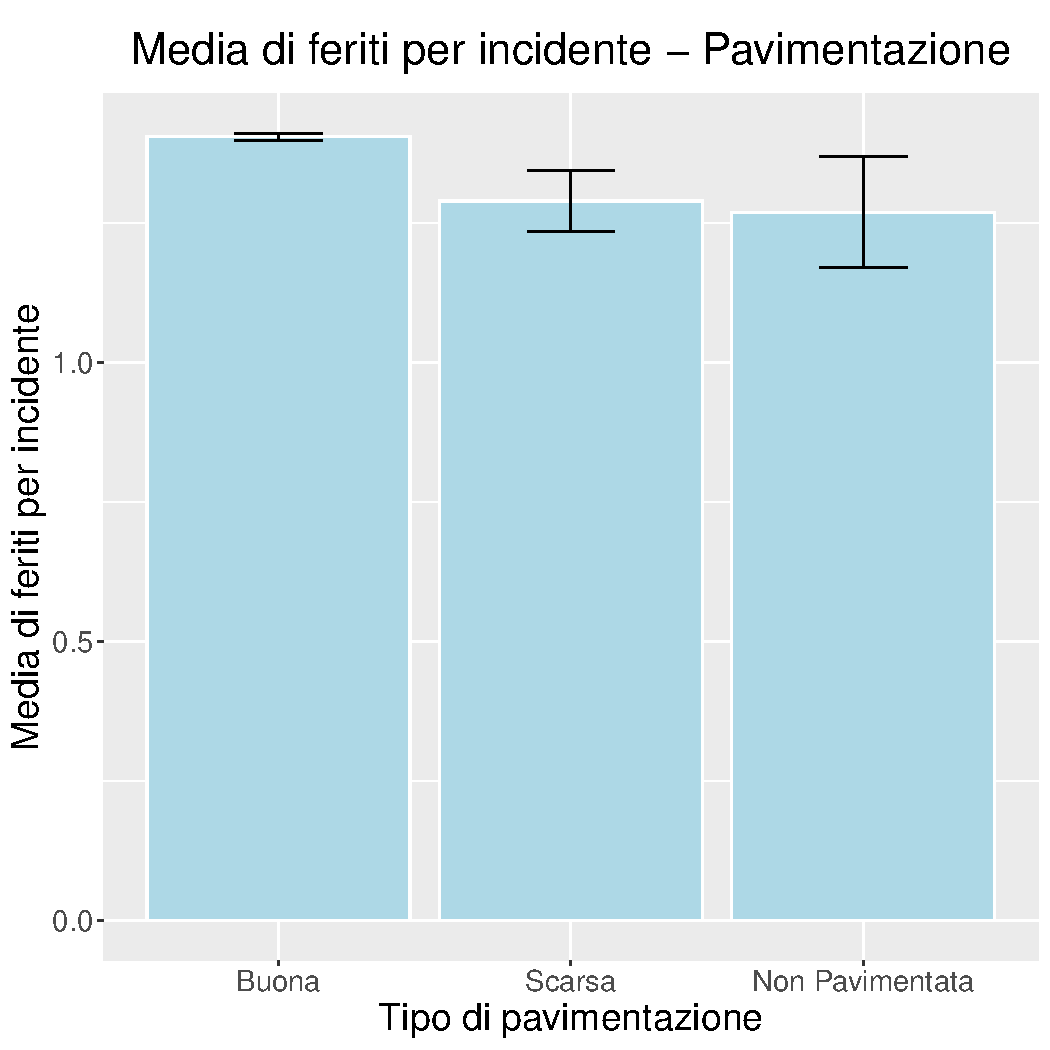
\includegraphics[scale=0.4]{../results/media_feriti_per_incidenti_pavimentazione.pdf}
            \end{subfigure}
            \hfill
            \begin{subfigure}{0.4\textwidth}
                \centering
                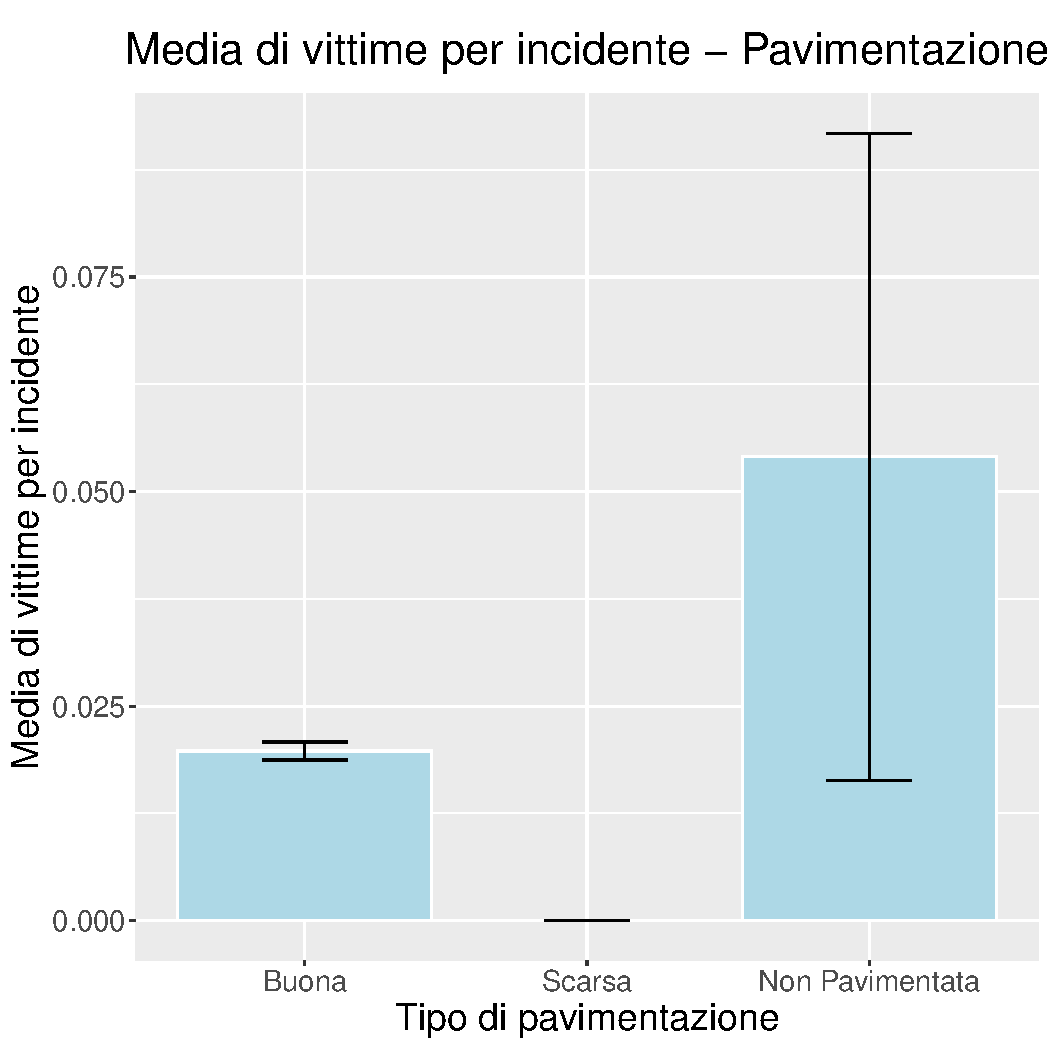
\includegraphics[scale=0.4]{../results/media_morti_per_incidenti_pavimentazione.pdf}
            \end{subfigure}
            \caption{Grafici a barre con il numero medio e la deviazione standard di feriti e morti per i diversi tipi di pavimentazione.}
            \label{Fig: morti_feriti_pavimentazione}
        \end{figure}   
        Si confronta attraverso un test d’ipotesi il numero di feriti per incidente con buona e scarsa pavimentazione:
        \begin{itemize}
            \item $H_0$: il numero medio di feriti per incidente stradale negli incidenti su strade pavimentate è uguale al numero di feriti per incidente su strade scarsamente pavimentate.
            \item $H_1$: il numero medio di feriti per incidente stradale negli incidenti su strade pavimentate è diverso  dal numero di feriti per incidente su strade scarsamente pavimentate.
            \item Confidence level: 99\%.
        \end{itemize}
        I risultati sono:
        \[
            Z_{test} = 1.486
        \]
        \[
            p-value = 0.137
        \]
        Il test non è statisticamente significativo. Non siamo in grado di rifiutare l’ipotesi nulla.
        
        Sempre in Figura \ref{Fig: morti_feriti_pavimentazione} viene illustrato il numero medio di vittime per incidente stradale condizionatamente al tipo di pavimentazione.
        
        Il test condotto confronta il numero di vittime per incidente su strada con buona pavimentazione e in assenza di pavimentazione.
        \begin{itemize}
            \item $H_0$: il numero medio di vittime per incidente stradale negli incidenti su strade pavimentate è uguale al numero di vittime per incidente su strade non pavimentate.
            \item $H_1$: il numero medio di vittime per incidente stradale negli incidenti su strade pavimentate è diverso  dal numero di vittime per incidente su strade non pavimentate.
            \item Confidence level: 99\%. 
        \end{itemize}
        In questo caso, si ha:
        \[
            Z_{test} = 1.973
        \]
        \[
            p-value = 0.0485
        \]
        Il test non è statisticamente significativo. Non possiamo rifiutare l’ipotesi nulla.
\clearpage

\section{Analisi Bivariata}
    \subsection{Confronto tra fondo stradale e tipo di strada}
        In questa sezione andiamo a vedere come il fondo stradale, ovvero se durante l'incidente esso fosse \textit{asciutto}, \textit{sdrucciolevole}, \textit{bagnato}, \textit{ghiacciato} o \textit{innevato}, possa incidere in maniera diversa a seconda della localizzazione dell'incidente, ovvero se esso sia su \textit{strada urbana}, \textit{strada extraurbana} oppure \textit{autostrada}.
    
        Per prima cosa abbiamo raggruppato nei tre gruppi descritti qua sopra le varie classificazioni di localizzazione incidente come riportate nel dataset dall'ISTAT.
        Inizialmente, oltre alla distinzione tra urbano, extraurbano e autostrada, veniva fatta una distinzione anche in base all'ente responsabile di tale strada, ovvero comune, provincia, regione o stato. Poiché al fine della nostra analisi questo non portava alcun tipo di informazione, abbiamo raggruppato.
        
        Come si può notare dalla Figura \ref{Fig: localizzazione_incidenti}, la maggior parte degli incidenti con feriti e/o morti sono localizzati in strade urbane.
        \begin{figure}[h]
            \centering
            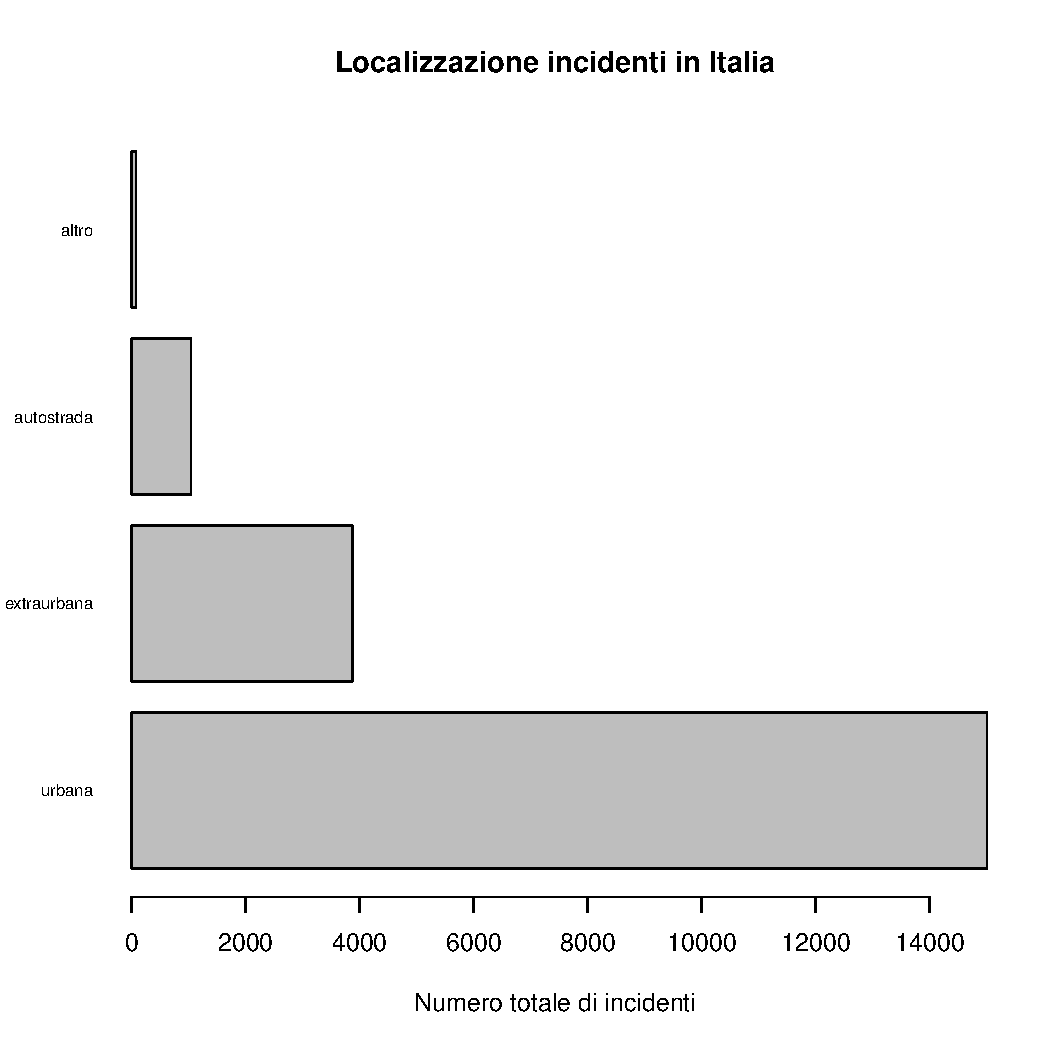
\includegraphics[scale=0.55]{../results/localizzazione_incidenti.pdf}
            \caption{Grafico a barre che mostra il numero di incidenti nelle varie localizzazioni stradali. }
            \label{Fig: localizzazione_incidenti}
        \end{figure}
        
        Successivamente, abbiamo però cercato di quantificare la pericolosità delle strade in base alla lunghezza totale di esse. Ovvero, siamo andati a vedere quanti fossero gli incidenti per chilometro di strada percorso. 
        
        Siamo riusciti solamente a ritrovare, dal sito web del \textit{Ministero dei Trasporti e delle Infrastrutture}, la lunghezza di tutte le strade Italiane (urbane e extraurbane insieme) e autostrade Italiane. Se da un lato siamo riusciti ad ottenere la pericolosità per chilometro percorso a seconda del tipo di strada, abbiamo perso precisione a causa dell’impossibilità, in questa istanza, di distinguere tra strade urbane e extraurbane.
        
        Come si può vedere in Figura \ref{Fig: localizzazione_incidenti_per_chilometro}, le autostrade risultano più pericolose per chilometro. 
        
        \begin{figure}[h]
            \centering
            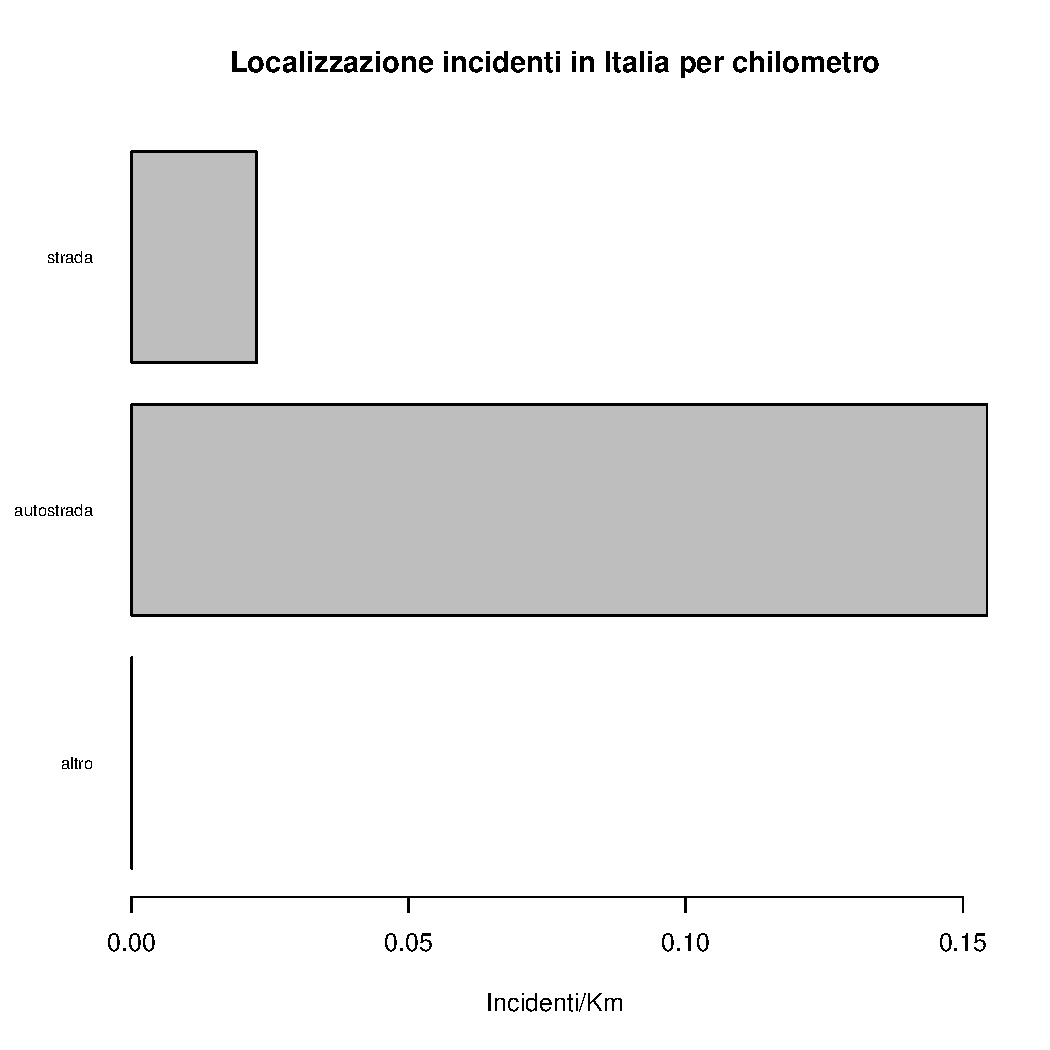
\includegraphics[scale=0.45]{../results/localizzazione_per_chilometro.pdf}
            \caption{Grafico a barre che mostra il numero di incidenti nelle varie localizzazioni stradali al km.}
            \label{Fig: localizzazione_incidenti_per_chilometro}
        \end{figure}
        
        Sebbene un risultato importante, questo non tiene conto della maggiore presenza di automobili sulle autostrade. Un'analisi completa dovrebbe quindi tenere conto del traffico presente, dati che non siamo stati in grado di procurarci.
        
        Come descritto sopra, siamo quindi andati a confrontare con i dati sulle condizioni del fondo stradale. 

        In Figura \ref{Fig: localizzazione_per_fondo} si mostra la localizzazione degli incidenti, con attenzione al fondo della strada al momento degli stessi. In Figura \ref{Fig: tabella_fondo_tipo} mostriamo invece le quantità di incidenti, sempre coi dati provenienti dal campione di 20000.
        \begin{figure}[h]
            \begin{subfigure}{0.4\textwidth}
                \centering
                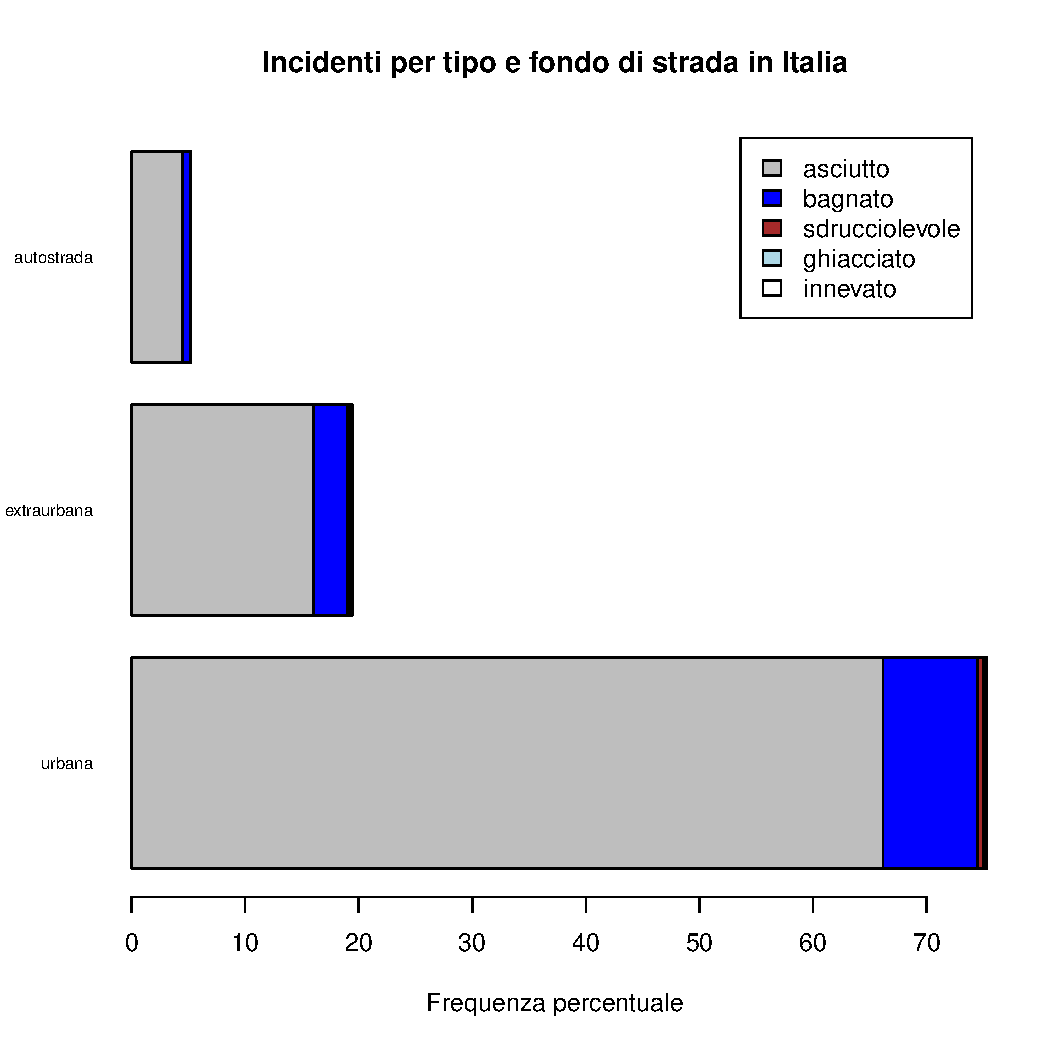
\includegraphics[scale=0.4]{../results/localizzazione_fondo.pdf}
                \caption{Grafico a barre per la localizzazione degli incidenti con specificazione, tramite diversi colori, del fondo stradale al momento dell'incidente. Come si può notare, fondo \textit{asciutto} e \textit{bagnato} sono praticamente gli unici distinguibili a occhio.}
                \label{Fig: localizzazione_per_fondo}
            \end{subfigure}
            \hfill
            \begin{subfigure}{0.4\textwidth}
                \centering
                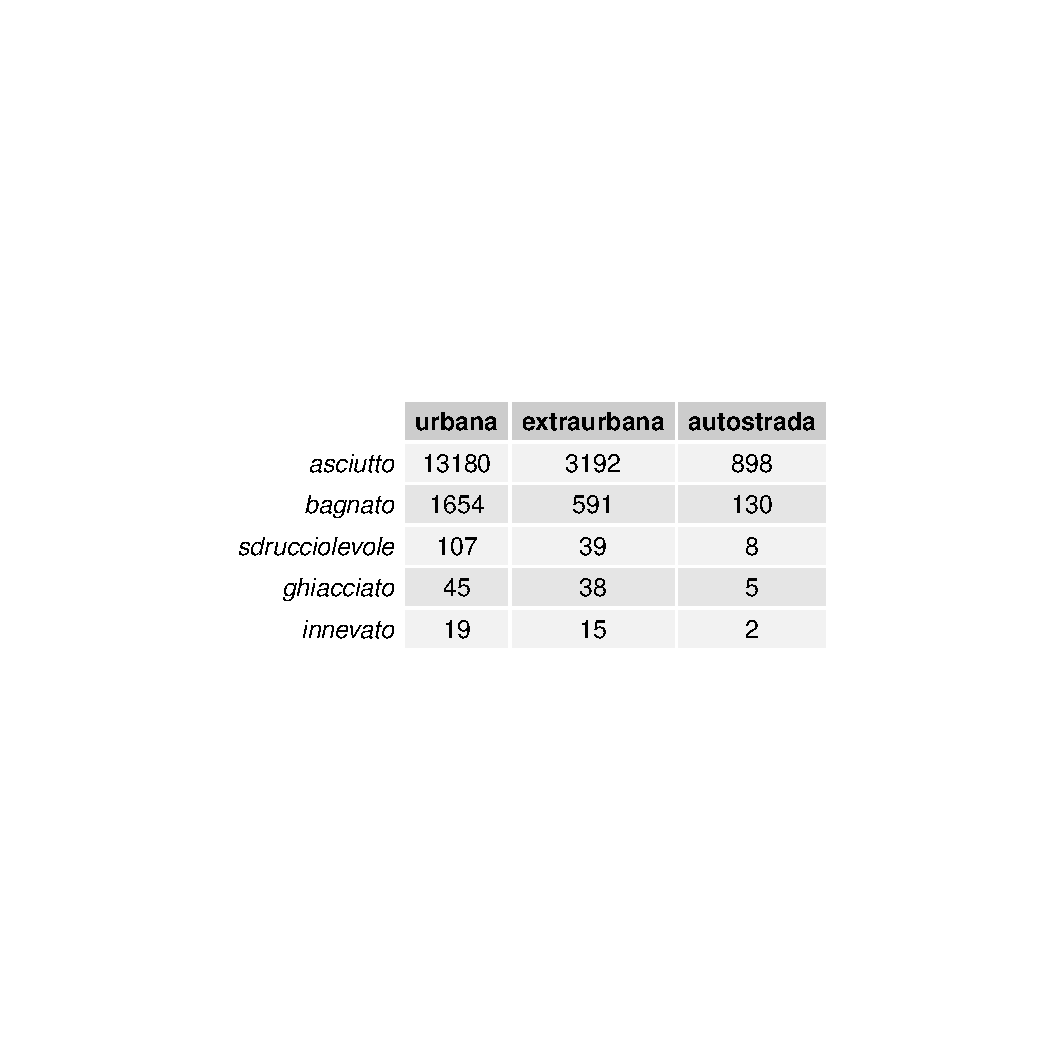
\includegraphics[scale=0.4]{../results/tabella_localizzazione_incidenti.pdf}
                \caption{Tabella a doppia entrata contenente le informazioni del grafico qua affianco. Si vede bene come, sul campione di 20000 incidenti, ben pochi accadano in presenza di fondo ``estremo", come \textit{innevato} o \textit{ghiacciato}.}
                \label{Fig: tabella_fondo_tipo}
            \end{subfigure}
            \caption{}
        \end{figure} 
        In dettaglio, siamo andati a calcolare la probabilità che il terreno bagnato potesse avere influenza sul tipo di strada. 
        \begin{itemize}
            \item Probabilità incidente causato da fondo bagnato in strada urbana 11.09 \%. 
            \item Probabilità incidente causato da fondo bagnato in strada extra urbana 16.78 \%.
            \item Probabilità incidente causato da fondo bagnato in autostrada 14.14 \%.
        \end{itemize}
        Una volta calcolate le probabilità associate ai 3 diversi tipi di strada, siamo andati a confrontarle al \textbf{livello di significatività} del 99\%. Per semplicità, siamo andati a eseguire dei test solamente a due a due, in modalità come descritto precedentemente, nella Sezione \ref{Sec: analisi_trimestrale}.
        
        Confrontando la presenza di \textbf{fondo bagnato} tra strada \textbf{urbana} e \textbf{extraurbana} si ottiene $Z = 3.71$. In questo caso, con il \textit{confidence level} dato, si ritiene il test passato: si ha dipendenza nell'effetto del fondo bagnato a seconda che l'incidente sia localizzato in una strada urbana o in una extraurbana. Ovvero, se vi è fondo bagnato, in una strada extraurbana si ha probabilità maggiore che accada un incidente.
        
        Viene ripetuto di seguito lo stesso calcolo confrontando strada urbana e autostrada con fondo bagnato, ottenendo un risultato di $Z = 1.14$. Con questo risultato e il \textit{confidence level} dato, non si può affermare che vi sia dipendenza tra i due. Questo potrebbe essere dovuto sia a vera indipendenza, sia a una limitazione dei dati a disposizione.
        
        Eseguendo lo stesso calcolo confrontando tra strada extraurbana e autostrada abbiamo ottenuto $Z = 0.80$. Anche qua, con il \textit{confidence level} dato non si può affermare che vi sia dipendenza fra i due fenomeni.
        
        In conclusione siamo in grado di affermare, con un confidence level del 99\%, che vi sia una maggiore probabilità che il fondo bagnato causi un incidente in una strada extraurbana rispetto a una urbana. Lo stesso non si può affermare per le altre coppie analizzate.
        
\clearpage
\section{Conclusione}
    Nel presente elaborato, abbiamo voluto delineare alcuni fattori di rischio legati alla guida di un autoveicolo su strade pubbliche, divenuta oramai un’azione abitudinaria per la maggior parte delle persone.
    
    Nella prima parte della relazione, abbiamo evidenziato quali sono gli orari in cui avvengono il maggior numero e il minor numero di incidenti.
    
    In seguito, abbiamo dato alcune indicazioni di tipo geografico, mettendo in evidenza l’autostrada più pericolosa, la città più pericolosa (anche in relazione al numero di abitanti) e, infine, le regioni più pericolose, sia dal punto di vista del numero di veicoli che del numero di patenti per regione.
    
    Queste prime indagini forniscono una visione grossolana della situazione degli incidenti in Italia, fornendo indicazioni di tipo temporale (orario) e spaziale (autostrade, città, regioni) sulle frequenze degli incidenti.
    
    In seguito, abbiamo preso in considerazione il numero di feriti e il numero di vittime per ciascun incidente, fornendo dei valori medi e degli indici di variabilità. L’obiettivo di questa sezione era quello di mettere in evidenza l’effettiva pericolosità degli incidenti con lesione. Si evince infatti che, nella grande maggioranza dei casi (oltre il 99\%), gli incidenti non causano alcuna vittima e che il numero di feriti supera raramente l’1.
    
    Abbiamo poi considerato gli incidenti in cui fosse coinvolto un solo veicolo, e li abbiamo suddivisi per genere del guidatore coinvolto. 
    Questa indagine aveva lo scopo di fornire una indicazione riguardante i responsabili degli incidenti a singolo veicolo, che, come si evince, sono per la maggior parte uomini.
    
    In seguito, abbiamo analizzato la pericolosità degli incidenti (intesa come numero di medio di feriti o vittime per singolo incidente) in funzione di vari fattori, come l’ora del giorno, il trimestre, il tipo di strada, il tipo di fondo stradale e la pavimentazione, determinando in quali casi si verificava un aumento della pericolosità. 
    
    Infine abbiamo valutato alcuni fattori di rischio relativi alla frequenza degli incidenti, effettuando una statistica bivariata che tenesse in considerazione il tipo di strada e il tipo di fondo stradale.
    Abbiamo poi effettuato dei test di ipotesi per determinare se ci fosse o no indipendenza fra i vari fattori.
    
    Attraverso le analisi condotte siamo stati in grado di fornire una prima visione d’insieme della situazione riguardante gli incidenti stradali in Italia. 
    Pur fornendo conclusioni utili, l’analisi risente della mancanza di alcune informazioni all’interno dei dataset, dovuti all’anonimizzazione dei dati, come ad esempio la data di ciascun incidente e il luogo geografico, che avrebbero reso il nostro lavoro più comprensivo.
    
    Ci auspichiamo quindi di poter approfondire l’indagine attraverso un’integrazione dati come quella appena descritta, servendoci anche di strumenti statistici più potenti. 
    Un esempio è costituito dalla possibilità di effettuare test d’ipotesi multipli applicando metodi di correzione del \textit{p-value}. 
    
    Pur soffrendo delle due mancanze appena descritte, riteniamo che il nostro lavoro possa comunque fornire una solida visione generale dei principali fattori di rischio legati agli incidenti stradali in Italia.

\end{document}
